\documentclass[a4paper,11pt]{article}
\usepackage[utf8]{inputenc}
\usepackage[margin=2cm]{geometry}

\usepackage{xcolor}
\definecolor{myblue}{rgb}{0.1 0.1 0.6}
% ``backref'' for drafting; see manual for further options
%\usepackage[backref]{hyperref}
%\usepackage{showkeys}
\usepackage{hyperref}
\hypersetup{
   colorlinks=true,
   linkcolor=myblue,
   citecolor=myblue,
   urlcolor=myblue
}

\usepackage[T1]{fontenc}
\usepackage{beton}
\usepackage[euler-digits, euler-hat-accent]{eulervm}
\DeclareFontSeriesDefault[rm]{bf}{sbc} 

\usepackage{amsmath,amssymb,amsthm}
%\usepackage[all]{xy}
\usepackage{url}
\usepackage[shortlabels]{enumitem}
%\usepackage{amscd}
\usepackage{tikz}
\usetikzlibrary{matrix,arrows}
\usepackage{tikz-cd}

\theoremstyle{plain}
\newtheorem{proposition}{Proposition}[section]
\newtheorem{theorem}[proposition]{Theorem}
\newtheorem{corollary}[proposition]{Corollary}
\newtheorem{lemma}[proposition]{Lemma}
\newtheorem{claim}[proposition]{Claim}
\newtheorem{definition}[proposition]{Definition}
\newtheorem{example}[proposition]{Example}
\newtheorem{question}[proposition]{Question}

\theoremstyle{remark}
\newtheorem{remarkx}[proposition]{Remark}
\newtheorem{remarksx}[proposition]{Remarks}
\newtheorem{workingx}[proposition]{Working}
% Some hacks to get a symbol printed at the end of a remark, as it was very unclear (in my
% writing style) where a remark ended and the general flow of the paper (re)started.
\newenvironment{remark}
  {\pushQED{\qed}\renewcommand{\qedsymbol}{$\triangle$}\remarkx}
  {\popQED\endremarkx}
\newenvironment{remarks}
  {\pushQED{\qed}\renewcommand{\qedsymbol}{$\triangle$}\remarksx}
  {\popQED\endremarksx}
\newenvironment{working}
  {\pushQED{\qed}\renewcommand{\qedsymbol}{$\triangle$}\workingx}
  {\popQED\endworkingx}


\newcommand{\mc}[1]{\mathcal{#1}}
\newcommand{\mf}[1]{\mathfrak{#1}}
\newcommand{\msf}[1]{\mathsf{#1}}

\newcommand{\ip}[2]{{\langle {#1} , {#2} \rangle}}
\newcommand{\lin}{\operatorname{lin}}
\newcommand{\id}{\operatorname{id}}

\newcommand{\vnten}{\bar\otimes}
\newcommand{\proten}{\widehat\otimes}

\newcommand{\hh}{\widehat}
\newcommand{\G}{\mathbb{G}}
\renewcommand{\H}{\mathbb{H}}
\newcommand{\op}{{\operatorname{op}}}
\newcommand{\im}{{\operatorname{Im}}}
\newcommand{\coker}{\operatorname{coker}}
\newcommand{\intdual}{\circledast}
\newcommand{\tr}{\operatorname{Tr}}
\newcommand{\ad}{{\operatorname{ad}}}
\newcommand{\lan}{\operatorname{Lan}}
\newcommand{\ran}{\operatorname{Ran}}

\begin{document}

\title{Interpolation spaces and duality}
\author{Matt Daws}
\date{May 2025}
\maketitle

\begin{abstract}
Some notes on the monograph by Kaijser and Pelletier.
\end{abstract}

\tableofcontents

\bigskip

We give some notes about the book \cite{KP_InterpolationFunctorsDuality}, written as the author was reading this book.  Part~I of the book makes a quick introduction to doolittle diagrams of Banach spaces, thought of as generalisations of Banach couples, and then shows how the ``real'' ($J$ and $K$ methods) and complex interpolation schemes can be introduced in this generalised setting.

The notes here currently give a detailed account of doolittle diagrams, but after that only cover selected topics.  I found the learning curve involved in thinking about doolittle diagrams to be steep, but once overcome, other parts of the book were not so hard to read.



\section{Doolittle Diagrams}

I find the discussion in Section~1 quite hard to follow, so here is a more pedestrian account.

The book works with the category of Banach spaces and bounded linear maps.  Often we might restrict to just contractive maps, giving a subcategory with generally nicer properties: for example, isomorphisms become isometric.  So ``operator'' will mean bounded linear map, unless stated otherwise.

\begin{definition}
A \emph{doolittle diagram} $\overline{X}$ of Banach spaces is a commutative diagram
\[ \begin{tikzcd}
\Delta\overline X \arrow[r, "\delta_0"] \arrow[d, "\delta_1"'] & X_0 \arrow[d, "\sigma_0"] \\
X_1 \arrow[r, "\sigma_1"'] & \Sigma\overline X
\end{tikzcd}
\]
which is both a pullback and a pushout.
\end{definition}

We recall from basic category theory (\cite[Definition~5.1.16]{Leinster_BasicCatTheory} for example) that $\Delta\overline X$ being the \emph{pullback} of $(\sigma_0, \sigma_1)$ means that whenever $Y$ is a Banach space with operators $f_0 \colon Y \to X_0, f_1 \colon Y \to X_1$ with $\sigma_0 f_0 = \sigma_1 f_1$, there is a unique operator $u\colon Y \to \Delta\overline X$ with $\delta_0 u = f_0, \delta_1 u = f_1$.  As a diagram:
\[ \begin{tikzcd}
Y \arrow[rd, dotted, "\exists !\, u"] \arrow[rrd, bend left, "f_0"] \arrow[rdd, bend right, "f_1"']\\
& \Delta\overline X \arrow[r, "\delta_0"] \arrow[d, "\delta_1"'] & X_0 \arrow[d, "\sigma_0"] \\
& X_1 \arrow[r, "\sigma_1"'] & \Sigma\overline X
\end{tikzcd}
\]

Similarly, that $\Sigma\overline X$ is the \emph{pushout} (\cite[Definition~5.2.11]{Leinster_BasicCatTheory} for example) of $(\delta_0, \delta_1)$ means that whenever $Z$ is a Banach space with operators $g_0 \colon X_0 \to Z$ and $f_1 \colon Z_1\to Z$ with $g_0\delta_0 = g_1\delta_1$, there is a unique operator $v\colon \Sigma\overline X \to Z$ with $v\sigma_0 = g_0, v\sigma_1=g_1$.  As a diagram:
\[ \begin{tikzcd}
\Delta\overline X \arrow[r, "\delta_0"] \arrow[d, "\delta_1"'] & X_0 \arrow[d, "\sigma_0"] \arrow[rdd, bend left, "g_0"] \\
X_1 \arrow[r, "\sigma_1"'] \arrow[rrd, bend right, "g_1"'] & \Sigma\overline X \arrow[rd, dotted, "v"] \\
&& Z    
\end{tikzcd} \]

Using the universal properties, it is routine to show that pullbacks and pushouts, if they exist, are unique up to isomorphism.

There are canonical constructions of these objects in the category of Banach spaces.  Firstly, for the pullback, define
\[ D(\sigma_0,\sigma_1) = D\sigma = \{ (\xi_0,\xi_1) : \sigma_0(\xi_0) = \sigma_1(\xi_1) \} \subseteq X_0 \oplus_\infty X_1. \]
As $\sigma_0,\sigma_1$ are continuous, $D\sigma$ is a closed subspace of $X_0 \oplus_\infty X_1$.
Let $\delta_i \colon D\sigma \to X_i$ be the natural projection maps restricted to $D\sigma$, which are contractions satisfying $\sigma_0\delta_0 = \sigma_1\delta_1$.
Given $Y, f_0, f_1$ as above, by definition, $(f_0(\xi), f_1(\xi)) \in D\sigma$ for each $\xi\in Y$ and so we obtain a map $u \colon Y \to D\sigma$.  Notice that $\|u(\xi)\| = \max( \|f_0(\xi)\|, \|f_1(\xi)\| ) \leq \|\xi\| \max(\|f_0\|, \|f_1\|)$ so $u$ is bounded, and contractive if $f_0,f_1$ both are.  Then $\delta_i u = f_i$ and so $u$ satisfies the required property.  Clearly $u$ is unique.  Hence $\Delta\overline X$ is isomorphic (but perhaps not isometric) with $D\sigma$.

For the pushout, set
\[ P(\delta_0,\delta_1) = P\delta = X_0 \oplus_1 X_1 / \overline\lin\{ (\delta_0(\xi), -\delta_1(\xi)) : \xi\in \Delta\overline X \}. \]
Notice that the linear span is superfluous, but the closure is needed, in general.  We shall abuse notation and suppress the quotient when writing elements of $P\delta$.
Let $\sigma_0(\xi_0) = (\xi_0,0)$ for $\xi_0\in X_0$, and simiarly define $\sigma_1(\xi_1) = (0,\xi_1)$ for $\xi_1\in X_1$; both of these operators are contractions.  For $\xi\in \Delta\overline X$ we see that $\sigma_0 \delta_0(\xi) = (\delta_0(\xi), 0) = (0, \delta_1(\xi)) = \sigma_1 \delta_1(\xi)$ by the choice of the subspace to quotient by.
Given $Z, g_0, g_1$ as above, define $v(\xi_0, \xi_1) = g_0(\xi_0) + g_1(\xi_1)$.  This is well-defined as $v(\delta_0(\xi), -\delta_1(\xi)) = g_0\delta_0(\xi) - g_1\delta_1(\xi) = 0$ for each $\xi\in\Delta\overline X$.  As we use the $1$-norm, $\|v\| \leq \max(\|g_0\|, \|g_1\|)$ and so $v$ is contractive if $g_0,g_1$ both are.  Finally, $v \sigma_0 = g_0$ and $v\sigma_1 = g_1$, 
and again $v$ is unique with these properties.  Hence $P\delta$ is the pushout, and so $\Sigma\overline X$ is isomorphic to $P\delta$.

\begin{remark}
We introduce some occasionally useful notation.  Given a subspace $E\subseteq X_0\oplus X_1$ let $E' = \{ (\xi_0, -\xi_1) : (\xi_0,\xi_1) \in E \}$.  (It will be clear from context that this can never be confused with a commutant.)  As the map $(\eta_0,\eta_1) \mapsto (\eta_0, -\eta_1)$ is an isometry, $(E')' = E$, and $E$ is closed if and only if $E'$ is closed.
\end{remark}

Of course, for a doolittle diagram we require compatibility between the constructions, in that we simultaneously have a pushout and a pullback.  The following is useful; we have not found an easily stated analogue starting with $P\delta$.
  
\begin{lemma}\label{lem:when_doolittle_from_pullback}
Let $X_0, X_1, F$ be Banach spaces, and $\sigma_i\colon X_i\to F$ operators, for $i=12$.  The diagram
\[ \begin{tikzcd}
D\sigma \arrow[r, "\delta_0"] \arrow[d, "\delta_1"'] & X_0 \arrow[d, "\sigma_0"] \\
X_1 \arrow[r, "\sigma_1"'] & F
\end{tikzcd} \]
is a doolittle diagram if and only if $\sigma_0(X_0) + \sigma_1(X_1) = F$.
\end{lemma}
\begin{proof}
By construction, $D\sigma = \{ (\xi_0,\xi_1) : \sigma_0(\xi_0) = \sigma_1(\xi_1) \}$ with $\delta_i$ being the projection maps.  As $D\sigma$ is closed, also $(D\sigma)'$ is closed, and so the space we quotient by in forming $P\delta$ is $\{ (\delta_0(\xi), -\delta_1(\xi)) : \xi\in D\sigma \} = \{ (\xi_0, -\xi_1) : (\xi_0,\xi_1) \in D\sigma \} = (D\sigma)'$, no closure required.

Let $F_0 = \sigma_0(X_0) + \sigma_1(X_1) \subseteq F$ a subspace (perhaps not closed) and define $\theta \colon F_0 \to P\delta =  X_0 \oplus_1 X_1 / (D\sigma)'$ by $\theta(\sigma_0(\xi_0) + \sigma_1(\xi_1)) = (\xi_0, \xi_1) + (D\sigma)'$.  This is well-defined, as
\begin{align*}
\sigma_0(\xi_0) + \sigma_1(\xi_1) = \sigma_0(\eta_0) + \sigma_1(\eta_1)
\quad&\Leftrightarrow\quad  \sigma_0(\xi_0-\eta_0) = -\sigma_1(\xi_1-\eta_1)  \\
&\Leftrightarrow\quad  (\xi_0-\eta_0, \xi_1-\eta_1) \in (D\sigma)'   \\
&\Leftrightarrow\quad  (\xi_0-\eta_0, \xi_1-\eta_1) = 0 \text{ in } P\delta   \\
&\Leftrightarrow\quad  (\xi_0, \xi_1) = (\eta_0, \eta_1) \text{ in } P\delta.
\end{align*}
So also $\theta$ is injective, and so by the Open Mapping Theorem, $\theta$ is an isomorphism if and only if $F_0$ is closed (as always $\theta$ is onto).  Let $\sigma'_i \colon X_i \to P\delta$ be the canonical maps, so $\sigma_0'(\xi_0) = (\xi_0,0) = \theta(\sigma_0(\xi_0))$ and similarly $\sigma_1' = \theta\circ\sigma_1$.  The result follows, as the required isomorphism between $F$ and $P\delta$ must be $\theta$.
\end{proof}

\begin{remark}\label{rem:when_equal_in_sigma}
As useful observation of this proof is that in $P\delta$, we have $(\xi_0,0) = (0,\xi_1)$ if and only if $(\xi_0, -\xi_1) \in (D\sigma)'$, if and only if $(\xi_0, \xi_1) \in D\sigma$.
\end{remark}

We now classify doolittle diagrams, up to isomorphism.

\begin{proposition}\label{prop:classification_doolittle}
Let $(X_0, X_1)$ be a pair of Banach spaces.  Given a closed subspace $E$ of $X_0 \oplus_\infty X_1$, setting $\delta_i \colon E \to X_i$ to be the restriction of the natural projection, we have that $\Delta\overline X = E$, and $\Sigma\overline X = P\delta$, gives a doolittle diagram.  Up to isomorphism, all doolittle diagrams arise in this way.
\end{proposition}
\begin{proof}
If $\overline X$ is a doolittle diagram, then $\Delta\overline X$ is isomorphic to $D\sigma$, the pullback of $(\sigma_0, \sigma_1)$.  By construction, $E = D\sigma$ is a closed subspace of $X_0 \oplus_\infty X_1$, and as above, $\Sigma\overline X$ is isomorphic to $P\delta$.

Conversely, given such an $E$, we construct $P\delta$.  To show we have a doolittle diagram, it remains to show that $E, \delta_0, \delta_1$ gives the pullback of $(\sigma_0, \sigma_1)$, these maps coming from the construction of $P\delta$.
%Notice that for any $\xi = (\xi_0, \xi_1) \in E$, we have $(\delta_0(\xi), \delta_1(\xi)) = (\xi_0, \xi_1) = \xi$.  It follows that $E_0 := \{ (\delta_0(\xi), -\delta_1(\xi)) : \xi\in\Delta\overline X\}$ is a closed subspace, as the map $(\eta_0,\eta_1) \mapsto (\eta_0, -\eta_1)$ is an isometry.  By the construction of $P\delta$, we now see that $\sigma_0(\xi_0) = \sigma_1(\xi_1)$ if and only if $(\xi_0, -\xi_1) \in E_0$.  That is, if and only if $(\xi_0,\xi_1) \in E$.  We conclude that $D\sigma = E$ isometrically, and the natural maps giving the pullback are $\delta_0,\delta_1$.  Hence we do obtain a doolittle diagram.
This follows immediately from Lemma~\ref{lem:when_doolittle_from_pullback}.
\end{proof}

Notice that the doolittle diagrams we construct from such closed subspaces $E$ have all the map $\delta_i, \sigma_i$ contractive.
If we work in the category of contractive maps, then this proposition classifies doolittle diagrams up to isometric isomorphism.  However, in general, we are free to renorm $D\overline X$ and $\Sigma\overline X$.  I believe that the comment at the bottom of Page~9 of \cite{KP_InterpolationFunctorsDuality} means that we only consider doolittle diagrams coming from this construction, and not renormings.

Henceforth, we shall assume doolittle diagrams arise \emph{isometrically} in this way, so $\Delta\overline X = D\sigma$ isometrically, and $\Sigma\overline X = P\delta$ isometrically.  By Proposition~\ref{prop:classification_doolittle}, we are free to choose $\Delta\overline X$ to be any closed subspace of $X_0\oplus_\infty X_1$, and then $\Sigma\overline X$ is uniquely determined.

Recall from e.g. \cite{BL_Interpolation_Sps_Book} that a \emph{Banach couple} is a pair of Banach spaces $(X_0, X_1)$ which are both realised as subspaces of a Hausdorff topological vector space.  This allows us to form the intersect $X_0 \cap X_1$ and sum $X_0 + X_1$ which then have natural norms
\[ \|\xi\|_{X_0 \cap X_1} = \max\big( \|\xi\|_{X_0}, \|\xi\|_{X_1} \big), \quad
\|\xi\|_{X_0+X_1} = \inf\{ \|\xi_0\|_{X_0} + \|\xi_1\|_{X_1} : \xi = \xi_0+\xi_1 \}. \]
Thus by definition $X_0 \cap X_1 \subseteq X_0 \oplus_\infty X_1$.  Let $\sigma_i \colon X_i \to X_0 + X_1$ be the inclusion maps, and notice that given $(\xi_0,\xi_1) \in X_0 \oplus_\infty X_1$, we have $\sigma_0(\xi_0) = \sigma_1(\xi_1)$ exactly when $\xi_0 = \xi_1$ in $X_0 \cap X_1$.  Hence $X_0 \cap X_1$ is the pullback of $(\sigma_0, \sigma_1)$ and Lemma~\ref{lem:when_doolittle_from_pullback} now shows that
\[ \begin{tikzcd}
X_0 \cap X_1 \arrow[r, "\delta_0"] \arrow[d, "\delta_1"'] & X_0 \arrow[d, "\sigma_0"] \\
X_1 \arrow[r, "\sigma_1"'] & X_0+X_1
\end{tikzcd} \]
is a doolittle diagram.

Notice that here $\sigma_0, \sigma_1$ are injective.  We shall see that this characterises Banach couples, but first we shall investigate the kernel of $\sigma_i$ in the general case.

\begin{lemma}\label{lem:kernels_maps}
For any doolittle diagram, we have that $\delta_0$ is injective on the kernel of $\delta_1$, and $\delta_0(\ker \delta_1) = \ker \sigma_0$.  Similarly $\delta_1(\ker \delta_0) = \ker \sigma_1$.
\end{lemma}
\begin{proof}
As $D\sigma$ is the pullback, we see immediately that
\[ \ker\delta_1 = \{ (\xi_0,\xi_1) \in D\sigma : \xi_1 = 0 \}
= \{ (\xi_0, 0) : \sigma_0(\xi_0) = 0 \}. \]
Obviously, if $(\xi_0,0) \in \ker\delta_1$ then $\delta_0((\xi_0,0)) = \xi_0$ and this is zero only when $(\xi_0,0) = 0$, so $\delta_0$ is injective on $\ker\delta_1$, and $\delta_0(\ker\delta_1) = \{ \xi_0\in X_0 : \sigma_0(\xi_0)=0 \} = \ker\sigma_0$.
\end{proof}

\begin{proposition}\label{prop:when_couple}
A doolittle diagram arises from a Banach couple if and only if $\sigma_0,\sigma_1$ are both injective.
\end{proposition}
\begin{proof}
As observed, Banach couples give rise to doolittle diagrams with $\sigma_0,\sigma_1$ injective.  Conversely, if $\sigma_0,\sigma_1$ are injective, then by the lemma, also $\delta_0,\delta_1$ are injective.  As $\sigma_0,\sigma_1$ are injective, we may use $\Sigma\overline X$ as our ambient space to form $X_0\cap X_1$ and $X_0 + X_1$.  Then $\xi_0 = \xi_1$ exactly when $(\xi_0,0) = (0,\xi_1)$ in $\Sigma\overline X$, that is, $(\xi_0,\xi_1) \in D\sigma$, see Remark~\ref{rem:when_equal_in_sigma}.  Hence $X_0 \cap X_1 = D\sigma$, isometrically.  The norm on $\Sigma\overline X = P\delta$ is then, for $\xi = \xi_0+\xi_1$,
\begin{align*}
\|\xi\| &= \inf\{ \|\eta_0\|_{X_0} + \|\eta_1\|_{X_1} : (\xi_0-\eta_0, \xi_1-\eta_1) \in (D\sigma)' \} \\
&= \inf\{ \|\eta_0\|_{X_0} + \|\eta_1\|_{X_1} : \xi_0-\eta_0 = \eta_1-\xi_1 \} \\
&= \inf\{ \|\eta_0\|_{X_0} + \|\eta_1\|_{X_1} : \xi = \xi_0 + \xi_1 = \eta_0 + \eta_1 \}
= \|\xi\|_{X_0 + X_1}.
\end{align*}
Thus $\Sigma\overline X = X_0+X_1$ isometrically.
\end{proof}

We shall call a doolittle \emph{classical} if it arises from a Banach couple.

\begin{remark}
Notice that $\sigma_0(\xi_0)=0$ if and only if $(\xi_0,0)=0 \in P\delta$ if and only if $(\xi_0,0) \in \Delta\overline X$.  Hence $\sigma_0$ is injective exactly when $(\xi_0,0) \in \Delta\overline X$ implies $\xi_0=0$ (this also follows from Lemma~\ref{lem:kernels_maps}).
As $\Delta\overline X \subseteq X_0\oplus_\infty X_1$ is a subspace, this is equivalent to $(\xi_0,\xi_1), (\xi_0',\xi_1) \in \Delta\overline X$ implies $\xi_0=\xi_0'$.

In this case, we can hence define $\alpha_1 \colon \delta_1(\Delta\overline X) \to X_0; \delta_1((\xi_0,\xi_1)) = \xi_1 \mapsto \xi_0$.  Thus actually $\alpha_1$ maps to $\delta_0(\Delta\overline X)$.  If $\sigma_1$ is injective, we have $\alpha_0 \colon \delta_0(\Delta\overline X) \to \delta_1(\Delta\overline X); \delta_0((\xi_0,\xi_1)) = \xi_0 \mapsto \xi_1$.  When both $\sigma_i$ are injective, the maps $\alpha_0, \alpha_1$ are mutual inverses: indeed, they are just the identity map on $X_0 \cap X_1$.

A standard way to obtain a Banach couple is to start with a contractive injection $\iota \colon X_0 \to X_1$.  Then $X_0 \cap X_1 = X_0$ isometrically, and $X_0 + X_1 = X_1$ isometrically, and the resulting doolittle diagram is
\[ \begin{tikzcd}
\Delta = X_0  \arrow[r, "="] \arrow[d, "\iota"'] & X_0 \arrow[d, "\iota"] \\
X_1 \arrow[r, "="'] & \Sigma = X_1
\end{tikzcd} \]

As a generalisation, consider a closed operator $T \colon X_0 \supseteq D(T) \to X_1$ and let $\Delta$ be the graph of $T$.  Then $\delta_0(\Delta) = D(T)$ and $\delta_0$ is clearly injective, so by Lemma~\ref{lem:kernels_maps}, $\sigma_1$ is injective.  Conversely, if $\sigma_1$ is injective, then we have $\alpha_0 \colon \delta_0(\Delta\overline X) \to \delta_1(\Delta\overline X)$ and its graph is equal to $\Delta\overline X$.
\end{remark}

By definition, in a doolittle diagram, we have that $\sigma_0\circ \delta_0 = \sigma_1 \circ \delta_1$.  Call this map $j \colon \Delta\overline X \to \Sigma\overline X$.  We say that $\overline X$ is \emph{non-trivial} when $j\not=0$.

\begin{proposition}\label{prop:when_j_zero}
We have that $\overline X$ is trivial, that is, $j=0$, if and only if $\Delta = Y_0 \oplus_\infty Y_1$ for closed subspaces $Y_i \subseteq X_i$.
\end{proposition}
\begin{proof}
If $\Delta = Y_0 \oplus_\infty Y_1$ then given any $\xi=(\xi_0,\xi_1)\in \Delta$ we see that also $(\xi_0,0) \in \Delta$ and so $(\xi_0,0) = 0$ in $\Sigma = P\delta$, see Remark~\ref{rem:when_equal_in_sigma}.  So $j(\xi) = \sigma_0 \delta_0(\xi)=0$.

Conversely, if $j=0$ then let $Y_0 = \{ \xi_0\in X_0 : (\xi_0,0)\in \Delta \}$ and similarly define $Y_1$.  Given $\xi=(\xi_0,\xi_1)\in \Delta$, as $0 = j(\xi) = \sigma_0(\xi_0) = (\xi_0,0) \in P\delta$ we have that $(\xi_0,0) \in \Delta$, and similarly $(0,\xi_1)\in\Delta$.  Hence $(\xi_0,\xi_1) \in Y_0 \oplus_\infty Y_1$, as claimed.
\end{proof}

Notice that in this case, $\Sigma = X_0/Y_0 \oplus_1 X_1/Y_1$.

To close this section, we discuss dual spaces.  By Hahn--Banach, we identify $(\Delta\overline X)^*$ with $X_0^* \oplus_1 X_1^* / \Delta^\perp$ and $(\Sigma\overline X)^*$ with $(\Delta')^\perp \subseteq X_0^* \oplus_\infty X_1^*$.  Furthermore, notice that $\sigma_i^* \colon (\Delta')^\perp \to X_i^*$ is the natural projection, and that $\delta_0^*(\xi_0^*) = (\xi_0^*,0) + \Delta^\perp$, and similarly for $\delta_1^*$.

\begin{proposition}\label{prop:dual}
Given a doolittle diagram $\overline X$, also the following is doolittle
\begin{equation} \begin{tikzcd}
(\Sigma\overline X)^* = (\Delta')^\perp  \arrow[r, "\sigma_0^*"] \arrow[d, "\sigma_1^*"'] & X_0^* \arrow[d, "\delta_0^*"]\\
X_1^* \arrow[r, "\delta_1^*"'] & (\Delta\overline X)^* = X_0^* \oplus_1 X_1^* / \Delta^\perp
\end{tikzcd} \label{eq:dual_doolittle_diagram}
\end{equation}
\end{proposition}
\begin{proof}
The only thing to check is that $X_0^* \oplus_1 X_1^* / \Delta^\perp = P(\sigma_0^*, \sigma_1^*)$.  This will follow if we show that $\Delta^\perp = ((\Delta')^\perp)'$.  However, $(\xi_0^*, \xi_1^*) \in ((\Delta')^\perp)'$ exactly when $\ip{(\xi_0^*, -\xi_1^*)}{(\xi_0,\xi_1)}=0$ for all $(\xi_0,\xi_1) \in \Delta'$, equivalently, $\ip{(\xi_0^*, -\xi_1^*)}{(\xi_0,-\xi_1)}=0$ for each $(\xi_0,\xi_1)\in \Delta$, that is, $(\xi_0^*, \xi_1^*) \in \Delta^\perp$, as the minus signs cancel.
\end{proof}

We write $\overline X^*$ for this doolittle diagram: the dual to $\overline X$.
We now see the usefulness of doolittle diagrams: these are closed under duality, but by Proposition~\ref{prop:when_couple}, we see that the dual doolittle diagram arises from a Banach couple only when $\delta_0^*$ and $\delta_1^*$ are injective, which is equivalent to $\delta_0,\delta_1$ both having dense range.  Furthermore, even if the dual is a Banach couple, the bidual is only a couple when $\sigma_0^*, \sigma_1^*$ have (norm) dense range, which seems even more restrictive.

With this in mind, we note that the bidual is
\[ \begin{tikzcd}
  ((\Delta')^\perp)')^\perp = \Delta^{\perp\perp} \arrow[r, "\delta_0^{**}"] \arrow[d, "\delta_1^{**}"'] & X_0^{**} \arrow[d, "\sigma_0^{**}"]\\
  X_1^{**} \arrow[r, "\sigma_1^{**}"] & X_0^{**} \oplus_1 X_1^{**} / (\Delta')^{\perp\perp}
\end{tikzcd} \]
The argument in the proof of the lemma shows that $((\Delta')^\perp)' = \Delta^\perp$ from which the identifications arise.  Notice that Hahn--Banach shows that $\Delta^{\perp\perp}$ is isometric to $\Delta^{**}$, and similarly $\Sigma(\overline X^{**}) = X_0^{**} \oplus_1 X_1^{**} / (\Delta')^{\perp\perp}$ is isometric to $(\Sigma\overline X)^{**}$.


\subsection{Morphisms}

\begin{definition}
A morphism of doolittle diagrams $\overline X \to \overline Y$ is a pair $T=(T_0, T_1)$ where $T_i\in\mc B(X_i, Y_i)$ making the following diagram commute:
\[ \begin{tikzcd} & X_0 \arrow[r, "T_0"] & Y_0 \arrow[rd, "\sigma_0"] \\
\Delta\overline X \arrow[ru, "\delta_0"] \arrow[rd, "\delta_1"'] & & &  \Sigma\overline Y \\
& X_1 \arrow[r, "T_1"'] & Y_1 \arrow[ru, "\sigma_1"'] \end{tikzcd} \]
\end{definition}

\begin{lemma}\label{lem:when_morphism}
A pair $T=(T_0,T_1)$ is a morphism if and only if $(\xi_0,\xi_1)\in\Delta\overline X$ implies that $(T_0(\xi_0), T_1(\xi_1)) \in \Delta\overline Y$.
\end{lemma}
\begin{proof}
Let $(\xi_0,\xi_1)\in\Delta\overline X$, so $\sigma_0 T_0 \delta_0(\xi_0,\xi_1) = (T_0(\xi_0), 0)$ and simiarly $\sigma_1 T_1 \delta_1(\xi_0,\xi_1) = (0, T_1(\xi_1))$.  Hence $T$ is a morphism exactly when $(T_0(\xi_0), T_1(\xi_1)) \in \Delta\overline Y$, see Remark~\ref{rem:when_equal_in_sigma}.
\end{proof}

Given a morphism $T$, write $\Delta T \colon \Delta\overline X \to \Delta\overline Y$ for the map given by the lemma.  We also obtain a map $\Sigma T \colon \Sigma\overline X \to \Sigma\overline Y$ as, given $(\xi_0,\xi_1) \in (\Delta\overline X)'$ also $(T_0(\xi_0), T_1(xi_1)) \in (\Delta\overline Y)'$, and hence we obtain a well-defined map $\Sigma T$.  We define the obvious norm,
\[ \|T\| = \max( \|T_0\|, \|T_1\| ). \]
When $\overline X$ arises from a Banach couple, the condition becomes that $T_0(\xi) = T_1(\xi)$ for each $\xi\in X_0 \cap X_1$, and hence we recover the usual notion of a morphism between couples, isometrically.

\begin{proposition}\label{prop:morphisms_as_pullback}
The morphism space $\overline X \to\overline Y$ is the pullback of the following diagram
\[ \begin{tikzcd}
  & \mc B(X_0, Y_0) \arrow[d, "\alpha_0"] \\
  \mc B(X_1,Y_1) \arrow[r, "\alpha_1"']  & \mc B(\Delta\overline X, \Sigma\overline Y)
\end{tikzcd} \]
where $\alpha_0(T_0)$ is the map $\Delta\overline X \to \Sigma\overline Y; (\xi_0,\xi_1) \mapsto (T_0(\xi_0), 0)$, and similarly for $\alpha_1$.
\end{proposition}
\begin{proof}
As before, the pullback is $\{ (T_0,T_1) : \alpha_0(T_0) = \alpha_1(T_1) \} \subseteq \mc B(X_0,Y_0) \oplus_\infty \mc B(X_1,Y_1)$.  We have that $\alpha_0(T_0) = \alpha_1(T_1)$ if and only if $(T_0(\xi_0),0) = (0,T_1(\xi_1))$ in $\Sigma\overline Y$ for each $(\xi_0,\xi_1)\in\Delta\overline X$, equivalently, $(T_0(\xi_0), T_1(\xi_1))\in\Delta\overline Y$.  So the result follows from Lemma~\ref{lem:when_morphism}.
\end{proof}

From Lemma~\ref{lem:when_morphism} it is clear that if $T\colon \overline X \to \overline Y$ and $S\colon \overline Y\to\overline Z$ then $S\circ T = (S_0\circ T_0, S_1\circ T_1)$ is a morphism $\overline X \to \overline Z$.

By taking adjoints of all the operators involved, compare Proposition~\ref{prop:dual}, it follows immediately that if $(T_0, T_1) \colon \overline X\to\overline Y$ then $(T_0^*, T_1^*) \colon \overline Y^* \to \overline X^*$.

Write $\kappa_X \colon X \to X^{**}$ for the canonical map from a Banach space to its bidual.

\begin{proposition}
The pair $(\kappa_{X_0}, \kappa_{X_1})$ is a morphism $\overline X \to \overline X^{**}$.
\end{proposition}
\begin{proof}
As above, we have $\Delta(\overline X^{**}) = (\Delta\overline X)^{\perp\perp}$.  The result is now immediate.
\end{proof}

Finally, we give another view of morphisms, showing that they can naturally be thought of as morphism of the doolittle diagrams; compare with the discussion in \cite[Section~IV.1]{KP_InterpolationFunctorsDuality}.

\begin{proposition}\label{prop:morphisms_of_diagrams}
A morphism $\overline X \to \overline Y$ may be described by four maps $\Delta T, T_0, T_1, \Sigma T$ making the following diagram commute:
\[ \begin{tikzcd}
\Delta\overline X \arrow[r, "\delta_0"] \arrow[d, "\delta_1"']
\arrow[rrr, bend left, "\Delta T"]
& X_0 \arrow[d, "\sigma_0"] \arrow[rrr, bend left, "T_0"]
& &
\Delta\overline Y \arrow[r, "\delta_0"] \arrow[d, "\delta_1"'] & Y_0 \arrow[d, "\sigma_0"]
\\
X_1 \arrow[r, "\sigma_1"'] \arrow[rrr, bend right, "T_1"']
& \Sigma\overline X \arrow[rrr, bend right, "\Sigma T"']
& &
Y_1 \arrow[r, "\sigma_1"'] & \Sigma\overline Y
\end{tikzcd}
\]
\end{proposition}
\begin{proof}
Given a morphism, we obtain maps $\Delta T$ and $\Sigma T$.  By construction, given $\xi = (\xi_0,\xi_1) \in \Delta\overline X$, we have $T_0 \delta_0(\xi) = T_0(\xi_0) = \delta_0 \Delta T(\xi)$.  Similarly for $\Sigma T$, and by definition of a morphism, the rest of the diagram commutes.

Conversely, given four maps making the diagram commute, we have by definition that $(T_0,T_1)$ forms a morphism.  Then that $T_0 \circ \delta_0 = \Delta_0 \circ \Delta T$ and similarly for $T_1$, we see that $\Delta T$ is uniquely determined by $(T_0,T_1)$.  Similarly for $\Sigma T$.
\end{proof}


\subsection{Constructions}

With reference to Lemma~\ref{lem:kernels_maps}, set $K_i\overline X = \ker(\sigma_i) \subseteq X_i$, so also $K_i\overline X = \delta_i(\ker \delta_{i+1})$ where ``$i+1$'' is interpretted modulo $2$.  The following is immediate.

\begin{lemma}\label{lem:defn_K}
Let $\Delta (K\overline X) = K_0\overline X \oplus_\infty K_1\overline X \subseteq X_0\oplus_\infty X_1$.  The following is a doolittle diagram, say $K\overline X$,
\[ \begin{tikzcd} \Delta(K\overline X) \arrow[r, "\delta_0"] \arrow[d, "\delta_1"'] & K_0\overline X \arrow[d] \\
K_1\overline X \arrow[r] & 0
\end{tikzcd} \]
where $\delta_i$ is the projection map, as usual, and the other maps are zero.
\end{lemma}

For the following, compare Proposition~\ref{prop:when_j_zero}.

\begin{proposition}\label{prop:Ki_and_j}
For any doolittle diagram, we have that
\[ K_0\overline X = \{ \xi_0\in X_0 : (\xi_0,0) \in \Delta\overline X \}, \quad
K_1\overline X = \{ \xi_1\in X_1 : (0,\xi_1) \in \Delta\overline X \} \]
and that $\ker j = \Delta(K\overline X) \subseteq \Delta\overline X$.
\end{proposition}
\begin{proof}
Again using Remark~\ref{rem:when_equal_in_sigma}, we see that $\sigma_0(\xi_0)=0$ if and only if $(\xi_0,0)=0$ in $P\delta$, if and only if $(\xi_0,0) \in \Delta\overline X$.  Similarly for $K_1\overline X$.

As $j(\xi_0,\xi_1) = \sigma_0\delta_0(\xi_0,\xi_1) = (\xi_0,0)$ we see that $j(\xi_0,\xi_1) = 0$ exactly when $(\xi_0,0) \in \Delta$.  Using that also $j=\sigma_1\delta_1$, we see that
\[ \ker j = \{ (\xi_0,\xi_1)\in \Delta : (\xi_0,0), (0,\xi_1) \in \Delta \}
= K_0\overline X \oplus_\infty K_1\overline X, \]
as claimed.
\end{proof}

The following shows how to convert a doolittle diagram into a Banach couple.

\begin{proposition}\label{prop:quotient_by_kernel}
For any doolittle diagram, the following is also a doolittle diagram $\overline X / K\overline X$
\[ \begin{tikzcd}
\Delta\overline X / \Delta(K\overline X) \arrow[r, "\hat\delta_0"] \arrow[d, "\hat\delta_1"'] & X_0 / K_0\overline X\arrow[d, "\hat\sigma_0"] \\
X_1 / K_1\overline X \arrow[r, "\hat\sigma_1"'] & \Sigma\overline X
\end{tikzcd}
\]
Here $\hat\delta_i$ is the quotient operator $\xi+K\overline X \mapsto \delta_i(\xi) + K_i\overline X$, and $\hat\sigma_i$ is the quotient operator $\xi_i + K_i\overline X \mapsto \sigma_i(\xi_i)$.  Further, the maps $\hat\sigma_i$ are injective, and so this diagram comes from a Banach couple.
\end{proposition}
\begin{proof}
As $\Delta(K\overline X) \subseteq \Delta\overline X$, the quotient exists, and as $\delta_i(\Delta(K\overline X)) \subseteq K_i\overline X$, the maps $\hat\delta_i$ are well-defined.  As $K_i\overline X = \ker\sigma_i$, similarly the maps $\hat\sigma_i$ are well-defined.  Clearly $\hat\sigma_i$ is injective.

Set $Y_i = X_i / K_i\overline X$ and $\Delta\overline Y = \{ (\xi_0', \xi_1') \in Y_0 \oplus_\infty Y_1 : \hat\sigma_0(\xi_0') = \hat\sigma_1(\xi_1') \}$.  As $\hat\sigma_0(Y_0) + \hat\sigma_1(Y_1) = \sigma_0(X_0) + \sigma_1(X_1) = \Sigma\overline X$, by Lemma~\ref{lem:when_doolittle_from_pullback}, the following is a doolittle diagram:
\[ \begin{tikzcd}
\Delta\overline Y \arrow[r, "\delta_0"] \arrow[d, "\delta_1"'] & Y_0 \arrow[d, "\hat\sigma_0"] \\
Y_1 \arrow[r, "\hat\sigma_1"'] & \Sigma\overline X
\end{tikzcd} \]
We see that for $(\xi_0,\xi_1)\in \Delta\overline X$ we have that $(\xi_0+K_0\overline X, \xi_1+K_1\overline X) \in \Delta\overline Y$, and the kernel of the resulting map $\Delta\overline X \to \Delta\overline Y$ is $K_0\overline X \oplus K_1\overline X = K\overline X$, while clearly this map is onto.  So $\Delta\overline X / \Delta(K\overline X) = \Delta\overline Y$ as Banach spaces.
Furthermore, in $\Delta\overline X / \Delta(K\overline X)$,
\begin{align*}
\| (\xi_0,\xi_1) + \Delta(K\overline X) \|
&= \inf\{ \max(\|\eta_0\|, \|\eta_1\|) : (\xi_0 - \eta_0, \xi_1-\eta_1) \in \Delta(K\overline X) \} \\
&= \inf\{ \max(\|\eta_0\|, \|\eta_1\|) : \xi_i - \eta_i \in K_i\overline X \} \\
&= \max( \|\xi_0+K_0\overline X\|, \|\xi_1+K_1\overline X\| ),
\end{align*}
as when computing the infimum we can let $\eta_0$ and $\eta_1$ vary independently.  Hence $\Delta\overline X / \Delta(K\overline X) = \Delta\overline Y$ isometrically, which completes the proof.
\end{proof}

By Proposition~\ref{prop:classification_doolittle}, a doolittle diagram only really depends upon $\Delta\overline X$, and there is some choice in $X_0,X_1$.  Indeed, we can always embed $X_i$ into larger spaces, leave $\Delta\overline X$ unchanged, and form a (larger) pullback to complete the diagram.  There is a construction to, in some sense, get around this problem.

Given $\Delta\overline X$ we set $X_i^\circ$ to be the closure of the image of $\delta_i$.  Then by construction, $\Delta\overline X$ is a closed subspace of $X_0^\circ \oplus_\infty X_1^\circ$, let $\Delta\overline X^\circ$ be this subspace, and so we obtain the doolittle diagram $\overline X^\circ$, namely
\[ \begin{tikzcd}
\Delta\overline X^\circ \arrow[r, "\delta_0"] \arrow[d, "\delta_1"'] & X_0^\circ \arrow[d, "\sigma_0"] \\
X_1^\circ \arrow[r, "\sigma_1"'] & \Sigma\overline X^\circ = X_0^\circ \oplus_1 X_1^\circ / (\Delta\overline X)'
\end{tikzcd} \]
The inclusion $X_0^\circ \oplus_1 X_1^\circ \to X_0\oplus_1 X_1$ drops to a map $\Sigma\overline X^\circ \to \Sigma\overline X$ which is isometric (as the space we quotient by is ``the same'').

[\footnote{Some stuff in the book about ``short exact sequences'' and quotients which we'll treat below in the category section.}]

By Lemma~\ref{lem:kernels_maps}, $\sigma_0,\sigma_1$ are injective if and only if $\delta_0,\delta_1$ are injective, so Proposition~\ref{prop:when_couple} shows that $\overline X^\circ$ comes from a Banach couple if and only if $\overline X$ does.  Recall that a Banach couple is \emph{regular} if $X_0\cap X_1$ is dense in both $X_0$ and $X_1$.  Thus the construction of $\overline X^\circ$ can be thought of as ensuring a regularity-like condition.

\begin{proposition}
We have that $K\overline X = K(\overline X^\circ)$, and that $(\overline X / K\overline X)^\circ$ is equal to $\overline X^\circ / (K\overline X)$.
\end{proposition}
\begin{proof}
Proposition~\ref{prop:Ki_and_j} gives that $K_0\overline X = \{ \xi_0\in X_0 : (\xi_0,0) \in \Delta\overline X \}$ and so $K_0\overline X \subseteq X_0^\circ$, and similarly for $K_1$.  Hence $K\overline X = K(\overline X^\circ)$.

Recall the doolittle diagram for $\overline X / K\overline X$ from Proposition~\ref{prop:quotient_by_kernel}.  As $\hat\delta_i$ is the quotient of $\delta_i$, we see that $(X_i / K_i\overline X)^\circ$ is the closure of $X_i^\circ / K_i\overline X$, but this is already closed as $K_i\overline X = K_i\overline X^\circ$.  It follows that $(\overline X / K\overline X)^\circ = \overline X^\circ / (K\overline X)$.
\end{proof}


\subsection{The resulting category}

Write $\msf{Ban}$ for the category of Banach spaces, $\msf{BanCp}$ for the category of Banach couples, and $\msf{BanDL}$ for the category of doolittle diagrams.  As discussed above, $\msf{BanCp}$ is a subcategory of $\msf{BanDL}$, in fact, it is a full subcategory.

We continue to be a little vague about whether we consider all (bounded) morphisms, or just contractive morphisms.  We will make comments about when the difference is important.  The following was written by the author, but much more detail can be found in \cite[Section~IV.3]{KP_InterpolationFunctorsDuality}.

We consider $\msf{BanDL}$ and the subcategory $\msf{BanCp}$.
The zero object in both these categories is the diagram with $X_0 = X_1 = \{0\}$ and the zero maps.  The zero morphisms are the pairs $(0,0)$.  The following is essentially \cite[Proposition~IV.3.2]{KP_InterpolationFunctorsDuality}.

\begin{proposition}\label{prop:kernel_DL}
Let $T=(T_0,T_1)$ be a morphism $\overline X \to \overline Y$.  We define $\ker T$ by setting $\Delta(\ker T) = \{ (\xi_0,\xi_1)\in\Delta\overline X : T_0(\xi_0)=0, T_1(\xi_1)=0 \}$.
Treat $\Delta(\ker T)$ as a subspace of $X_0\oplus_\infty X_1$, so that we obtain doolittle diagram $\ker T$.  With $\iota$ given by the formal identity, we obtain a morphism $\ker T \to \overline X$ which is the categorical kernel of $T$.
\end{proposition}
\begin{proof}
Let $\iota_i \colon X_i\to X_i$ be the identity, so $\iota$ is a morphism as $\Delta(\ker T) \subseteq \Delta\overline X$ by definition.
Suppose we have a diagram
\[ \begin{tikzcd}
  \overline X \arrow[rd, "T"] \\
  \overline Z \arrow[u, "S"] \arrow[r, "0"'] & \overline Y
\end{tikzcd} \]
We show the existence of a unique morphism $\phi\circ \overline Z \to \ker T$ with $S = \iota\circ \phi$.  As $T_i\circ S_i = 0$, given $(\eta_0,\eta_1) \in \Delta\overline Z$ we have that $(S_0(\eta_0), S_1(\eta_1)) \in \Delta\overline X$ as $S$ is a morphism, and $(T_0S_0(\eta_0), T_1S_1(\eta_1))= (0,0)$ so $(S_0(\eta_0), S_1(\eta_1)) \in \Delta(\ker T)$.  Thus we can consider $\phi_i$ as $S_i$, giving a morphism $\phi\colon\overline Z \to \ker T$ with $\iota\circ\phi=S$.  As $\iota$ is the formal identity, clearly $\phi$ is uniquely defined.
\end{proof}

It might be more notationally consistent to write $\overline{\ker T}$ or $\overline\ker T$, but it should be clear from context that if $T$ is a morphism of doolittle diagrams, then $\ker T$ is a doolittle diagram with ``inclusion'' morphism.
As kernels are unique (up to isomorphism) we don't have any choice in this construction: in particular, notice that we only change the $\Delta$ space to form the kernel.  We can similarly construct cokernels; once one unpacks the construction, this agrees with \cite[Proposition~IV.3.2]{KP_InterpolationFunctorsDuality}.

\begin{proposition}\label{prop:cokernel_DL}
Let $T=(T_0,T_1)$ be a morphism $\overline X \to \overline Y$.  We define $\coker T$ to be the doolittle diagram with pair of spaces $Q_i = Y_i / \overline{T_i(X_i)}$ with natural quotient maps $q_i \colon Y_i \to Q_i$, and $\Delta(\coker T)$ to be the closure of the image of $\Delta Y$, namely the closure of $\{ (q_0(\xi_0), q_1(\xi_1)) : (\xi_0,\xi_1)\in\Delta Y \}$.  Then $q$ gives a morphism $\overline Y \to \coker T$, and this gives the categorical cokernel.
\end{proposition}
\begin{proof}
By construction, $q$ is a morphism, and $q \circ T = 0$.  Let $\overline Q'$ be a doolittle diagram with morphism $q' \colon Y \to \overline Q'$ with $q' \circ T = 0$.  We show the existence of a unique morphism $\phi \colon \coker T \to \overline Q'$ with $\phi\circ q = q'$.

Define $\phi_i \colon q_i(\xi_i) = q_i'(\xi_i)$, which is well-defined, as if $q_i(\xi_i)=0$ then $\xi_i\in \overline {T_i(X_i)}$ and so $q_i'(\xi_i)=0$.  Given $(\xi_0,\xi_1) \in \Delta\overline Y$, we have that $(q_0(\xi_0), q_1(\xi_1)) \in \Delta(\coker T)$ and $(\phi_0q_0(\xi_0), \phi_1q_1(\xi_1)) = (q'_0(\xi_0), q'_1(\xi_1)) \in \Delta\overline Q'$.  By density of such elements in $\Delta(\coker T)$, it follows that $\phi$ is a morphism, with $\phi\circ q = q'$ by construction.  As $q_i$ is onto, $\phi_i$ is uniquely defined, and so $\phi$ is unique.
\end{proof}

This construction suggests a general notion of a ``quotient''.  First we need the notion of a ``subspace''; this should be compared with the arguably better definition below, Definition~\ref{defn:subspace_quotient}.

\begin{definition}\label{defn:old_subspace_quotient}
Let $\overline X$ be a doolittle diagram.  A \emph{subspace} of $\overline X$ is $\overline Y$ where $Y_i\subseteq X_i$ are closed subspaces, and $\Delta Y \subseteq \Delta X$.

The \emph{quotient} is $\overline Q = \overline X / \overline Y$ where $Q_i = X_i / Y_i$ and $\Delta\overline Q$ is the closure of the image of $\Delta\overline X$ in $Q_0 \oplus_\infty Q_1$.  Let $q_i \colon X_i \to Q_i$ be the quotient map.
\end{definition}

\begin{proposition}
The subspace and quotient form doolittle diagrams, with the inclusion $\overline Y\to\overline X$ a morphism, and $q=(q_0,q_1) \colon \overline X \to \overline X/\overline Y$ a morphism.
\end{proposition}
\begin{proof}
The subspace is by definition a doolittle diagram, and obviously the inclusion gives a morphism, as $\Delta Y \subseteq \Delta X$ by definition.  Again, the quotient is doolittle by definition, and $\Delta Q$ is defined so that $q$ forms a morphism.
\end{proof}

The quotient construction has the following universal property.

\begin{proposition}\label{prop:factor_through_quotient}
Let $\overline Y$ be a subspace of $\overline X$.  The quotient $Q = \overline X / \overline Y$ has the property that a morphism $T\colon \overline X \to \overline Z$ factors through $q\colon \overline X \to \overline Q$ if and only if $Y_i \subseteq \ker(T_i)$ for $i=0,1$.
\end{proposition}
\begin{proof}
If we have $T$ and $S\colon\overline Q\to\overline Z$ with $S\circ q = T$, then for $\xi_i\in Y_i$ we have that $T(\xi_i) = S_i q_i(\xi_i) = 0$, so $Y_i \subseteq \ker(T_i)$.  Conversely, if this holds, then define $S_i \colon X_i / Y_i \to Z_i$ by $S_i(\xi_i + Y_i) = T_i(\xi_i)$, which is well-defined by the assumption that $T_i(Y_i) = \{0\}$.  Then $\|S_i\| \leq \|T_i\|$, and for $(\xi_0,\xi_1) \in \Delta\overline X$ we see that $(\xi_0+Y_0, \xi_1+Y_1) \in \Delta\overline Q$ and $(S_0(\xi_0+Y_0), S_1(\xi_1+Y_1)) = (T_0(\xi_0), T_1(\xi_1)) \in \Delta\overline Z$.  By the density of such elements in $\Delta\overline Q$, we conclude that $S$ is a morphism.  By construction, $S\circ q = T$.
\end{proof}

\begin{remark}
It seems strange that the quotient does not depend upon $\Delta\overline Y$.  However, firstly, the factorisation property given by Proposition~\ref{prop:factor_through_quotient} only holds because $\Delta Q$ is minimal, in the sense that the image of $\Delta X$ is dense.  Indeed, let $\overline Q'$ be a doolittle diagram with $Q'_i = X_i / Y_i$ but $\Delta\overline Q'$ arbitrary with $\Delta \overline Q' \supseteq \overline Q$.  The quotient map $q'$ is still a morphism.  However, $q \colon \overline X \to \overline Q$ does not factor through $q'$ unless $\Delta\overline Q' \subseteq \Delta\overline Q$, that is, actually $\overline Q' = \overline Q$.

Of course, perhaps requiring some extra property from $T$ would give an alternative formulation of this factorisation property, using a different notion of quotient.
\end{remark}

\begin{remark}
Continuing, consider how we might somehow use $\Delta\overline Y$ in defining the quotient.  It is perhaps natural to try to use $\Delta\overline X / \Delta\overline Y$ as the pullback.  This would mean a doolittle diagram like
\[ \begin{tikzcd}
\Delta\overline X / \Delta\overline Y \arrow[r, "\delta_0"] \arrow[d, "\delta_1"'] & X_0/Y_0 \arrow[d, "\sigma_0"] \\
X_1/Y_1 \arrow[r, "\sigma_1"'] & P\delta
\end{tikzcd}
\qquad\text{where}\quad
P\delta = (X_0/Y_0 \oplus_1 X_1/Y_1) / \{ (\delta_0\xi,-\delta_1\xi) : \xi\in \Delta\overline X / \Delta\overline Y \}^{\overline{\phantom{\{\ }}^{\|\cdot\|}}. \]
Of course, this means that $\Delta\overline X / \Delta\overline Y \cong D\sigma$ where
\begin{align*}
D\sigma &= \{ (\xi_0+Y_0, \xi_1+Y_1) : \sigma_0(\xi_0+Y_0) = \sigma_1(\xi_1+Y_1) \}  \\
&= \{ (\xi_0+Y_0, -\xi_1+Y_1) : (\xi_0+Y_0, -\xi_1+Y_1) = 0 \in P\delta \} \\
&= \{ (\delta_0\xi,\delta_1\xi) : \xi\in \Delta\overline X / \Delta\overline Y \}^{\overline{\phantom{\{\ }}^{\|\cdot\|}}.
\end{align*}
We need to decide on the maps $\delta_i$, for which the natural choice seems to be $\delta_0 \colon \overline X / \overline Y \to X_0/Y_0; (\xi_0,\xi_1)+\overline Y \mapsto \xi_0+Y_0$, and similarly for $\delta_1$.  These are well-defined, for if $(\xi_0,\xi_1)\in\overline Y$ then $\xi_0\in Y_0$ and $\xi_1\in Y_1$.  For these choices,
\[ D\sigma = \{ (\xi_0+Y_0, \xi_1+Y_1) : (\xi_0,\xi_1)\in\Delta\overline X \}^{\overline{\phantom{\{\ }}^{\|\cdot\|}}, \]
and we're back to $\Delta\overline Q$.

Thus an arbitrary $\Delta\overline Y$ doesn't seem to work.  For which $\Delta\overline Y$ do we have that $\Delta\overline X / \Delta\overline Y \cong \Delta\overline Q$?  The natural map to use is $\Delta\overline X / \Delta\overline Y \ni (\xi_0,\xi_1) + \Delta\overline Y \mapsto (\xi_0+Y_0, \xi_1+Y_0) \in \Delta\overline Q$, which has dense range.  It is injective if and only if $(\xi_0,\xi_1)\in\Delta\overline X \cap Y_0\oplus Y_1 \subseteq \Delta\overline Y$, but as $\Delta\overline Y \subseteq \Delta\overline X$ and $Y_0\oplus Y_1$, we must have equality:
\[ \Delta\overline Y = \Delta\overline X \cap Y_0\oplus Y_1. \]
We also require the map to be bounded below (ideally, to be an isometry).  For $(\xi_0,\xi_1) \in \Delta\overline X$, the two norms are
\begin{gather*}
\|(\xi_0,\xi_1)\|_{\Delta\overline X / \Delta\overline Y}
= \inf\big\{ \max(\|\xi_0-\eta_0\|, \|\xi_1-\eta_1\|) : (\eta_0,\eta_1) \in \Delta\overline X \cap Y_0\oplus Y_1 \big\}, \\
\|(\xi_0,\xi_1)\|_{\Delta\overline Q}
= \inf\big\{ \max(\|\xi_0-\eta_0\|, \|\xi_1-\eta_1\|) : (\eta_0,\eta_1) \in Y_0\oplus Y_1 \big\}.
\end{gather*}
It seems hard to give a characterisation of when this happens.

However, in the special case that $\Delta\overline X \cap Y_0\oplus Y_1 = Y_0 \oplus Y_1$, we obviously do have equality.  This occurs for $K\overline X$, see Lemma~\ref{lem:defn_K}.
\end{remark}

A related issue occurs with our notion of a subspace: do we also have that $\Sigma Y \to \Sigma X$ is an ``inclusion'', which we might take to mean, ``is isometric''?  This is again rare, because while we always have a contractive map (compare Proposition~\ref{prop:morphisms_of_diagrams}), for $(\xi_0,\xi_1) \in Y_0\oplus Y_1$ we have
\begin{gather*}
\|(\xi_0,\xi_1)\|_{\Sigma\overline Y}
= \inf\big\{\max(\|\xi_0-\eta_0\|, \|\xi_1-\eta_1\|) : (\eta_0,\eta_1)\in \Delta\overline Y\big\}, \\
\|(\xi_0,\xi_1)\|_{\Sigma\overline X}
= \inf\big\{\max(\|\xi_0-\eta_0\|, \|\xi_1-\eta_1\|) : (\eta_0,\eta_1)\in \Delta\overline X\big\}.
\end{gather*}
A case when we do have equality is in the construction of $\overline X^\circ$, for the boring reason that there $\Delta\overline X^\circ = \Delta\overline X$.

In \cite[Section~I.2]{KP_InterpolationFunctorsDuality}, the notion of a \emph{short exact sequence} of couples is defined, by requiring that all the four maps (Proposition~\ref{prop:morphisms_of_diagrams}) are exact at each point of the diagram.  While the constructions $\overline X\mapsto K\overline X$ and $\overline X \mapsto \overline X^\circ$ give examples, it seems hard to think of other cases, given the discussion just made.


\subsection{Interpolation}

Classically, given a Banach couple $(X_0, X_1)$, an interpolation space is simply a Banach space $X$ with $X_0\cap X_1 \subseteq X \subseteq X_0+X_1$ (continuous inclusions) such that for every morphism $T$, there is a bounded operator $X\to X$ extending the map on $X_0\cap X_1$.

For a doolittle diagram, the map $j\colon \Delta\overline X \to \Sigma\overline X$ need not be injective, and so the notion of interpolation is more subtle.  For doolittle diagrams $\overline X, \overline Y$ write $\mc B(\overline X,\overline Y)$ for the morphism space, and write $\mc B(\overline X)$ for $\mc B(\overline X,\overline X)$.

The most basis idea is simply that of a $\mc B(\overline X)$-module, equivalently, a Banach space $X$ with a homomorphism $\mc B(\overline X) \to \mc B(X)$.  As always, we have a choice as to whether this homomorphism is assumed contractive, or just bounded.  We can always re-norm $X$ to be contractive, by setting
\[ \| x \|_0 = \sup\{ \|T\cdot x \| : T\in\mc B(\overline X), \|T\|\leq 1 \}. \]
As $1\in\mc B(\overline X)$ acts as the identity on $X$, this norm is equivalent to the given norm.  We see that for $\|T\|\leq $, for $S\in\mc B(\overline X)$ with $\|S\|\leq 1$ also $\|ST\|\leq 1$ and so $\|T\cdot x\|_0 = \sup\{ \|ST\cdot x\| : \|S\|\leq 1 \} \leq \sup\{ \|R\cdot x\| : \|R\|\leq 1 \} = \|x\|_0$, as required to show that the module action for $\|\cdot\|_0$ is contractive.

\begin{definition}\label{defn:int_space}
Let $\overline X$ be a doolittle diagram.  We call an $\mc B(\overline X)$-module a \emph{quasi-interpolation space} for $\overline X$ if additionally there are module maps $\delta \colon \Delta\overline X \to X$ and $\sigma\colon X\to\Sigma\overline X$ with $\sigma\circ\delta = j$.  When $\delta$ has dense range, we call $X$ a \emph{$\Delta$-interpolation space}.  When $\sigma$ is injective, we call $X$ a \emph{$\Sigma$-interpolation space}.
\end{definition}

Notice that $X = \Delta\overline X$ gives a $\Delta$-interpolation space (which is only a $\Sigma$-interpolation space when $j$ is injective).  Similarly $X = \Sigma\Delta$ give a $\Sigma$-interpolation space (which is only a $\Delta$-interpolation space when $j$ is injective).

If $X$ is a $\Delta$-interpolation space, then $\delta$ being a dense-range module maps shows that the $\mc B(\overline X)$-module action on $X$ is uniquely defined.  Similarly for a $\Sigma$-interpolation space.

\cite{KP_InterpolationFunctorsDuality} observes that most $\Delta$-interpolation spaces are also $\Sigma$-interpolation spaces, but \cite[Example~I.3.2]{KP_InterpolationFunctorsDuality} shows that this isn't always so (an example different from $X = \Delta\overline X$).



\section{Part II Category theory}

\cite[Part~II]{KP_InterpolationFunctorsDuality} is concerned with category theory aspects.  I find it easier to read than Part~I, probably because of the work put in to understand Part~I.  So initial theory of abstract doolittle diagrams in general categories is expounded, but here we shall just look at Banach spaces.  Much more explictly, both the book, and these notes, now work with morphisms being contractions, not arbitrary bounded linear maps (unless specified).

\subsection{Morphism spaces and tensor products}\label{sec:mor_tenprod}

Recall that $\msf{Ban}$ is a ``closed category'', in particular, has an internal Hom functor, or in down to Earth language, $\mc B(X,Y)$ is itself a Banach space.  Notice that, if we restrict to morphisms being contractions, then this is not actually the Hom space.  Similarly we have the projective tensor product, and the relation that $\mc B(X, \mc B(Y,Z)) \cong \mc B(X\proten Y, Z)$.

We have already turned $\mc B(\overline X,\overline Y)$ into a Banach space.  Notice that Proposition~\ref{prop:morphisms_as_pullback} shows, in particular, that the norm we placed on $\mc B(\overline X, \overline Y)$ agrees with the norm on the pullback.  We now define a doolittle diagram representing the morphism space $\overline X \to \overline Y$, denoted $\overline{\mc B}(\overline X,\overline Y)$.  We define $\Delta\overline B \subseteq \mc B(X_0,Y_0) \oplus_\infty \mc B(X_1, Y_1)$ to be $\mc B(\overline X, \overline Y)$, and then complete to a doolittle diagram
\[ \begin{tikzcd}
\Delta\overline B \arrow[r, "\delta_0"] \arrow[d, "\delta_1"'] & \mc B(X_0,Y_0) \arrow[d, "\sigma_0"] \\
\mc B(X_1,Y_1) \arrow[r, "\sigma_1"'] & \Sigma\overline B
\end{tikzcd} \]
Here $\delta_i$ is the natural projection map, and $\Sigma\overline B$ is the pushforward, so explicitly
\[ \Sigma\overline B = \big( \mc B(X_0,Y_0) \oplus_1 \mc B(X_1,Y_1) \big)
/ \{ (T_0, -T_1) :  (T_0, T_1) \in \mc B(\overline X, \overline Y) \}. \]

We similarly define tensor products.  Given $\overline X,\overline Y \in \msf{BanDL}$ we define $\overline X \proten \overline Y \in \msf{Ban}$ to be the pushout of
\[ \begin{tikzcd}
  \Delta\overline X \proten \Delta\overline Y \arrow[r, "p_0"] \arrow[d, "p_1"'] & X_0 \proten Y_0 \\ X_1\proten Y_1
\end{tikzcd} \]
Here $p_i \colon (\xi_0,\xi_1) \otimes (\eta_0,\eta_1) \mapsto \xi_i \otimes \eta_i$.  That is,
\begin{equation} \overline X \proten \overline Y = \big(  (X_0 \proten Y_0) \oplus_1 ( X_1 \proten Y_1) \big) / \big\{ (p_0(u), -p_1(u)) : u \in \Delta\overline X \proten \Delta\overline Y \big\}^{\overline{\phantom{x}}^{\|\cdot\|}}. \label{eq:dl_tenprod}
\end{equation}
As usual, let $\sigma_i \colon X_i\proten Y_i \to \overline X \proten \overline Y$ be the usual maps.  As $\overline X \proten \overline Y$ is defined as a pushout, it satisfies the universal property that if $Z$ is any Banach space with contractive maps $g_i \colon X_i\proten Y_i \to Z$ satisfying $g_0p_0 = g_1p_1$, there is a unique contraction $\psi \colon \overline X\proten\overline Y \to Z$ with $g_i = \psi \sigma_i$.  As in Banach space theory, describing maps to $\overline X \proten \overline Y$ is harder.

The associated doolittle diagram, denoted $\overline X \overline{\proten} \overline Y$, is obtained by setting $\Sigma(\overline X \overline{\proten} \overline Y) = \overline X \proten \overline Y$, and defining $\Delta$ to be the pullback, giving
\begin{equation} \begin{tikzcd}
\Delta(\overline X \overline{\proten} \overline Y) \arrow[r, "\delta_0"] \arrow[d, "\delta_1"'] & X_0 \proten Y_0 \arrow[d, "\sigma_0"] \\ X_1\proten Y_1 \arrow[r, "\sigma_1"'] & \Sigma(\overline X \overline{\proten} \overline Y) = \overline X \proten \overline Y
\end{tikzcd}
\label{eq:tenprod_full_dl}
\end{equation}
By construction, the maps $p_i$ satisfy that $\sigma_0p_0 = \sigma_1p_1$ and so by the universal property of the pullback, there is a unique $\phi \colon \Delta\overline X \proten \Delta\overline X \to \Delta(\overline X \overline\proten \overline Y)$ with $\delta_i \circ \phi = p_i$.  Indeed, $\Delta(\overline X \overline\proten \overline Y)$ is by definition the subspace of $(X_0\proten Y_0)\oplus_\infty(X_1\proten Y_1)$ consisting of pairs $(u_0,u_1)$ with $\sigma_0(u_0) = \sigma_1(u_1)$.  Equivalently, $(u_0, -u_1) = 0$ in the quotient space $\overline X \proten \overline Y$ given by \eqref{eq:dl_tenprod}.  The map $\phi$ is simply $u\mapsto (p_0(u), p_1(u))$, and as the subspace we quotient by is generated by such pairs (up to a minus sign) we conclude that $\phi$ has dense range.  We remark that it seems hard to give a more concrete description of $\Delta(\overline X \overline{\proten} \overline Y)$, since it seems that $\phi$ need not be an isometry, or even bounded below, in general.

We shall generally suppress the map $\phi$ and regard $\Delta\overline X \otimes \Delta\overline Y$ as a dense subspace of $\Delta(\overline X \overline{\proten} \overline Y)$: notice that $\phi$ restricted to the algebraic tensor product is certainly injective.  The following proof illustrates this point of view.

\begin{proposition}\label{prop:tenprod_morphisms}
Let $\overline T \colon \overline X \to \overline Z$, and $\overline S \colon \overline Y \to \overline W$ be morphisms.  Then there is a morphism $\overline T \otimes \overline S \colon \overline X \overline{\proten} \overline Y \to \overline Z \overline{\proten} \overline W$ which has components $T_i\otimes S_i \colon X_i\proten Y_i \to Z_i\proten W_i$.  The resulting map of Banach spaces
\[ \overline T \otimes \overline S \colon \overline X \proten \overline Y \to \overline Z \proten \overline W \]
is uniquely determined by the relations $(\overline T \otimes \overline S) \sigma_i = \sigma_i (T_i \otimes S_i)$, with $\sigma_i$ as in \eqref{eq:tenprod_full_dl}.
\end{proposition}
\begin{proof}
If $\overline T, \overline S$ are contractive, then so are $T_i\otimes S_i \colon X_i\proten Y_i \to Z_i\proten W_i$.  We need to check that we map $\Delta(\overline X \overline{\proten} \overline Y)$ to $\Delta(\overline Z \overline{\proten} \overline W)$.  It suffices to prove that we map $\Delta\overline X \otimes \Delta\overline Y$ to $\Delta\overline Z \otimes \Delta\overline W$, but this is clear, as the required map is simply $\Delta\overline T \otimes \Delta\overline S$.
\end{proof}

More generally we can describe $\mc B(\overline X\overline\proten\overline Y, \overline Z)$.

\begin{proposition}\label{prop:tensor_adjoint_hom}
Let $T_i \colon X_i\proten Y_i \to Z_i$ for $i=0,1$.  Then $\overline T=(T_0,T_1)$ is a morphism $\overline X\overline\proten\overline Y \to \overline Z$ if and only if, for each $x=(x_0,x_1)\in\Delta\overline X, y=(y_0,y_1)\in\Delta\overline Y$ we have $(T_0(x_0\otimes y_0), T_1(x_1\otimes y_1)) \in \Delta\overline Z$.  We have that $\mc B(\overline X\overline\proten\overline Y, \overline Z) \cong \mc B(\overline X, \overline{\mc B}(\overline Y,\overline Z))$.
\end{proposition}
\begin{proof}
We again use the dense-range map $\phi \colon \Delta\overline X \otimes \Delta\overline Y \to \in\Delta(\overline X\overline\proten\overline Y)$.  That $\Delta\overline T$ exists is, by continuity, equivalent to $(T_0,T_1)\phi(\Delta\overline X \otimes \Delta\overline Y) \subseteq \Delta\overline Z$.  This is now immediately seen to be equivalent to the statement in the claim.

Given a morphism $\overline T\colon \overline X\overline\proten\overline Y \to \overline Z$ we define $\overline S=(S_0,S_1) \colon \overline X \to \overline{\mc B}(\overline Y,\overline Z)$ by setting $S_i \colon X_i \to \mc B(Y_i, Z_i)$ to be $S_i(x_i)(y_i) = T_i(x_i\otimes y_i)$.  Then $\Delta\overline S$ exists as given $(x_0,x_1)\in\Delta\overline X$, we claim that $(S_0(x_0), S_1(x_1)) \in \Delta \overline{\mc B}(\overline Y,\overline Z)$.  That is, for $(y_0,y_1)\in\Delta\overline Y$, we have that $(S_0(x_0)(y_0), S_1(x_1)(y_1))\in\Delta\overline Z$, but this is immediate as $\overline T$ has this property.  This argument is easily reversed to show that every $\overline S \in \mc B(\overline X, \overline{\mc B}(\overline Y,\overline Z))$ arises in this way.
\end{proof}

More is in \cite[Section IV.2]{KP_InterpolationFunctorsDuality}.



\subsection{Morphisms and inclusions}

We start by considering isomorphisms in $\msf{BanDL}$.

\begin{proposition}\label{prop:isomorphism_DL}
In $\msf{BanDL}$, $T=(T_0,T_1) \colon \overline X \to \overline Y$ is an isomorphism if and only if $T_0,T_1$ are both isomorphisms of Banach spaces, and given $(\xi_0,\xi_1) \in X_0\oplus_\infty X_1$ we have that $(\xi_0,\xi_1) \in \Delta\overline X$ if and only if $(T_0\xi_0, T_1\xi_1) \in \Delta\overline Y$.
\end{proposition}
\begin{proof}
By definition, $T$ is an isomorphism if and only if there is a morphism $S$ with $ST = 1_{\overline X}$ and $TS = 1_{\overline Y}$.  If so, then $T_i$ is invertible with $S_i = T_i^{-1}$, and that $S$ is a morphism shows that $(\eta_0, \eta_1) = (T_0\xi_0, T_1\xi_1) \in \Delta\overline Y$ implies $(\xi_0,\xi_1) = (S_0\eta_0, S_1\eta_1)\in\Delta\overline X$.  Conversely, if $T_0,T_1$ are isomorphisms with the condition of the $\Delta$ spaces, then $S = (T_0^{-1}, T_1^{-1})$ is a morphism $\overline Y\to\overline X$ forming the inverse to $T$.
\end{proof}

The following are easily proved from the definitions.

\begin{proposition}\label{prop:monomorphism_DL}
For $T\colon\overline X\to\overline Y$, the following are equivalent:
\begin{enumerate}
  \item $T$ is a monomorphism (so given $S\colon\overline Z\to\overline X$ if $T\circ S = 0$ then $S=0$);
  \item $T_0, T_1$ are injective;
  \item $T_0, T_1$ and $\Delta T$ are injective;
  \item $\ker T = \overline{0}$ (see Proposition~\ref{prop:kernel_DL}).
\end{enumerate}
\end{proposition}

\begin{proposition}\label{prop:epimorphism_DL}
For $T\colon\overline X\to\overline Y$, the following are equivalent:
\begin{enumerate}
  \item $T$ is an epimorphism (so given $S\colon\overline Y\to\overline Z$ if $S\circ T = 0$ then $S=0$);
  \item $T_0, T_1$ have dense range;
  \item $T_0, T_1$ and $\Sigma T$ have dense range;
  \item $\coker T = \overline{0}$ (see Proposition~\ref{prop:cokernel_DL}).
\end{enumerate}
\end{proposition}

The following are made as \emph{definitions} in \cite[Definition~3.5]{KP_InterpolationFunctorsDuality} but we wish to stress that they are results.  We state this in the case when morphisms are contractive, but in general one may replace ``isometry'' by ``bounded below''.

\begin{proposition}\label{prop:ex_monomorphism_DL}
For $T\colon\overline X\to\overline Y$, the following are equivalent:
\begin{enumerate}
  \item $T$ is an extremal monomorphism (which means that if $T = S\circ R$ with $R$ an epimorphism, then necessarily $R$ is an isomorphism);
  \item $T_0$ and $T_1$ are isometries, and $\Sigma T$ is injective.
\end{enumerate}
In this case, also $\Delta T$ is an isometry.
\end{proposition}
\begin{proof}
If $T_0,T_1$ are isometries, then also $\Delta T$ will be.  Notice that
\[ \Sigma T \colon \Sigma\overline X = X_0\oplus_1 X_1 / (\Delta\overline X)' \to 
\Sigma\overline Y = Y_0\oplus_1 Y_1 / (\Delta\overline Y)', \quad (\xi_0,\xi_1) + (\Delta\overline X)' \mapsto (T_0\xi_0, T_1\xi_1) + (\Delta\overline Y)' \]
is injective exactly when $(T_0\xi_0, T_1\xi_1) \in \Delta\overline Y$ implies that $(\xi_0,\xi_1) \in \Delta\overline X$ (the minus signs again cancelling).

Suppose that $T_0,T_1$ are isometries and that $\Sigma T$ is injective, and that $T = S\circ R$ with $R$ an epimorphism.  Then $T_i = S_i \circ R_i$ and $R_i$ has dense range, so that $T_i$ is an isometry shows that $R_i$ is isometric, and hence $R_i$ is an isometric isomorphism.  We verify the remaining condition from Proposition~\ref{prop:isomorphism_DL}, so let $(T_0\xi_0, T_1\xi_1) \in \Delta\overline Y$.  By assumption, then $(\xi_0,\xi_1) \in \Delta\overline X$, exactly the condition we need to show that $T$ is an isomorphism.

Conversely, let $T$ be an extremal monomorphism.  Set $Z_i = \overline{ T_i(X_i) } \subseteq Y_i$ and define $\Delta\overline Z = \Delta\overline Y \cap (Z_0\oplus_\infty Z_1)$, so we obtain a doolittle diagram $\overline Z$.  We can define $R_i \colon X_i \to Z_i$ to be the corestriction of $T_i$, and $\iota_i \colon Z_i\to Y_i$ to be the inclusion.  Then $R$ and $\iota$ are morphisms, and $\iota\circ R = T$.  As $R_i$ has dense range, $R$ is an epimorphism, and so $R$ is an isomorphism.  Hence $R_i$, so also $T_i$, is an isometry, and if $(R_0\xi_0, R_1\xi_1) \in \Delta Z$ then $(\xi_0,\xi_1) \in \Delta X$.  So, if $(T_0\xi_0, T_1\xi_1) \in \Delta Y$, then by construction of $\Delta Z$, also $(R_0\xi_0, R_1\xi_1) \in \Delta Z$, so $(\xi_0,\xi_1) \in \Delta X$, and we have checked that $\Sigma T$ is injective.
\end{proof}

\begin{remark}
Performing the calculations, it seems very unlikely that $\Sigma T$ will be an isometry, though I do not have a counter-example.

The method of proof here suggests what the ``closed image'' of $T$ should be, namely $\overline Z$.
\end{remark}

We analogously have the epimorphism version, which is the following.  A ``metric surjection'' is a surjective linear map $T\colon X\to Y$ with $\|y\| = \inf\{ \|x\| : T(x)=y \}$ for each $y\in Y$, that is, such that the induced map $\hat T \colon X/\ker T \to Y$ is an isometric isomorphism.  Again, if our category has morphisms as all bounded linear maps, then one can replace ``metric surjection'' by ``quotient map'' (that $\hat T$ is an isomorphism).

\begin{proposition}\label{prop:ex_epimorphism_DL}
For $T\colon\overline X\to\overline Y$, the following are equivalent:
\begin{enumerate}
  \item $T$ is an extremal epimorphism (which means that if $T = S\circ R$ with $S$ a monomorphism, then necessarily $S$ is an isomorphism);
  \item $T_0$ and $T_1$ are metric surjections, and $\Delta T$ has dense range.
\end{enumerate}
In this case, also $\Sigma T$ is a metric surjection.
\end{proposition}
\begin{proof}
If $T_0, T_1$ are metric surjections, then clearly $T_0 \oplus T_1 \colon X_0\oplus_1 X_1 \to Y_0\oplus_1 Y_1$ is also a metric surjection.  As quotient maps are metric surjections, it follows readily that $\Sigma T$ is also a metric surjection.

Suppose that $T_0, T_1$ are metric surjections, and that $\Delta T$ has dense range.  Let $T = S\circ R$, for some $S\colon\overline Z\to\overline Y$, and with each $S_i$ injective.  Then each $S_i$ is surjective, and so is an isomorphism.  For $\eta_i \in Y_i$ and $\epsilon>0$ there is $\xi_i\in X_i$ with $\|\xi_i\| < \|\eta_i\| + \epsilon$ and with $T\xi_i = \eta_i$.  Set $\alpha_i = R_i\xi_i$ so $S_i \alpha_i = \xi_i$ and hence $\alpha_i$ is unique with this property.  Furthermore, $\|\eta_i\| = \|S_i\alpha_i\| \leq \|\alpha_i\| = \|R_i\xi_i\| \leq \|\xi_i\| < \|\eta_i\| + \epsilon$ so $\|\alpha_i\| \leq \|\xi_i\| < \|\alpha_i\|+\epsilon$.  As $\epsilon>0$ was arbitrary, $\|\alpha_i\| = \|\xi_i\|$ and so $S_i$ is isometric.

We again verify the condition of Proposition~\ref{prop:isomorphism_DL}.  Given $(S_0\alpha_0, S_1\alpha_1) \in \Delta\overline Y$, as $\Delta T$ has dense range, we can approximate by $(T_0\xi_0, T_1\xi_1)$ for some $(\xi_0,\xi_1) \in \Delta\overline X$.  As $S_0, S_1$ are isometries, it follows that $(\alpha_0,\alpha_1)$ is approximated by $(R_0\xi_0, R_1\xi_1)$ which is in $\Delta\overline Z$, so as this is closed, also $(\alpha_0,\alpha_1) \in \Delta\overline Z$.  So $S$ is an isomorphism.

Conversely, let $T$ be an extremal epimorphism.  Set $Q_i = X_i / \ker T_i$, let $q_i \colon X_i\to Q_i$ be the quotient map, and set $\delta\overline Q$ to the closure of $\{ (q_0\xi_0, q_1\xi_1) : (\xi_0,\xi_1) \in \Delta\overline X \}$. Then $\overline Q$ is a doolittle diagram and $q\colon\overline X \to \overline Q$ a morphism.  Let $S_i \colon Q_i \to Y_i$ be induced by $T_i$, and notice that $\Delta\overline Q$ is constructed so that $S$ gives a morphism $\overline Q\to\overline Y$.  Then $S\circ q = T$ and as each $S_i$ is injective, $S$ is a monomorphism, and so $S$ is an isomorphism.

As each $S_i$ is an isometric isomorphism, by definition, each $T_i$ is a metric surjection.  Given $(\eta_0, \eta_1)\in\Delta\overline Y$, let $(\alpha_0,\alpha_1) = (S_0^{-1}\eta_0, S_1^{-1}\eta_1) \in \Delta\overline Q$.  We can approximate this as $(q_0\xi_0, q_1\xi_1)$ for $(\xi_0,\xi_1)\in\Delta\overline X$, and then by continuity, $(T_0\xi_0, T_1\xi_1) = (S_0q_0\xi_0, S_1q_1\xi_1)$ approximates $(\alpha_0, \alpha_1)$.  Thus $\Delta T$ has dense range.
\end{proof}

Again, it seems rather unlikely that $\Delta T$ need by surjective.

Motivated by these results, we can define subspaces and quotients.

\begin{definition}\label{defn:subspace_quotient}
Let $\overline X$ be a doolittle diagram.  If $\overline Y$ is doolittle with $Y_i \subseteq X_i$ a closed subspace, we say that $\overline Y$ is a \emph{subspace} of $\overline X$ when the inclusion $\iota\colon\overline Y\to\overline X$ is an extremal monomorphism.

A \emph{(metric) surjection} is an extremal epimorphism $\overline X \to \overline Y$.
\end{definition}

So $\overline Y \subseteq \overline X$ is a subspace when $Y_i \subseteq X_i$ is a closed subspace, $\iota$ is a morphism, and $\Sigma\iota$ is injective.  That $\iota$ is a morphism means that $\Delta\overline Y \subseteq \Delta\overline X$, where we regard $Y_0\oplus_\infty Y_1 \subseteq X_0\oplus_\infty X_1$.  That $\Sigma\iota$ is injective means that if $(\iota_0\xi_0, \iota_1\xi_1) \in \Delta\overline X$, then $(\xi_0,\xi_1) \in \Delta\overline Y$.  That is, we must have $\Delta\overline Y = \Delta\overline X \cap (Y_0 \oplus_\infty Y_1)$; we have hence shown \cite[Proposition~3.8]{KP_InterpolationFunctorsDuality}.

Consider now an extremal epimorphism $T \colon \overline X \to \overline Y$.  Up to isometric isomorphism, we have that $Y_i = X_i / \ker T_i$, and that $\{ (\xi_0+\ker T_0, \xi_1+\ker T_1) : (\xi_0,\xi_1) \in \Delta\overline X\}$ is a dense subspace of $\Delta\overline Y$.  Equivalently, $\Delta\overline Y$ is the closure of this subspace of $Y_0 \oplus_\infty Y_1$.  This accords with our previous definition of a quotient, Definition~\ref{defn:old_subspace_quotient}.


\subsection{Finite-rank morphisms}

We say that $\overline X \in \msf{BanDL}$ is \emph{finite-dimensional} if $X_0,X_1$ are.  A morphism $\overline T \colon \overline X \to \overline Y$ is \emph{finite-rank} if $T$ factors through a finite-dimensional doolittle diagram; see \cite[Section~V.3]{KP_InterpolationFunctorsDuality}.

\begin{proposition}
We have that $\overline T \colon \overline X \to \overline Y$ is finite-rank if and only if $T_0,T_1$ are finite-rank operators $X_i\to Y_i$.
\end{proposition}
\begin{proof}
If $\overline T$ is finite-rank, then $T_0, T_1$ factor through finite-dimensional Banach spaces, and so have finite-rank.  Conversely, if $T_0, T_1$ are finite-rank operators, then set $Z_i = T_i(X_i) \subseteq Y_i$ finite-dimensional subspaces.  Let $\overline Z$ be the subspace induced, so $\Delta\overline Z = \Delta\overline Y \cap (Z_0 \oplus\infty Z_1)$.  That $\overline T$ is a morphism means that for $(\xi_0, \xi_1) \in \Delta\overline X$ we have that $(T_0\xi_0, T_1\xi_1) \in \Delta\overline Y \cap (Z_0 \oplus Z_1) = \Delta\overline Z$, and so $\overline T$ corestricts to a morphism $\overline S \colon \overline X\to\overline Z$.  With $\iota\colon \overline Z \to \overline Y$ the inclusion, we have our factorisation $\overline T = \iota \circ \overline S$.
\end{proof}

The following is from \cite[Section~IV.2]{KP_InterpolationFunctorsDuality}.  Recall the map $j = \sigma_0\delta_0 = \sigma_1\delta_1 \colon \Delta\overline X \to \Sigma\overline X$.

\begin{definition}
An element $u\in\Delta\overline X$ is a \emph{unit} if $\|ju\| = \|u\| = 1$.  If $\|j\|=1$ then $\overline X$ has an \emph{approximate unit}, a sequence of unit vectors $(u_n)$ in $\Delta\overline X$ with $\|j(u_n)\| \to 1$.
\end{definition}

\begin{lemma}
Let $u$ be a unit for $\overline X$.  There is $u^* \in (\Sigma\overline X)^*$ with $\|u^*\| = 1 = \ip{u^*}{ju}$ and then $u^*$ is a unit for $\overline X^*$.
\end{lemma}
\begin{proof}
We recall the dual doolittle diagram from Proposition~\ref{prop:dual}.  That $u^*$ exists is the Hahn--Banach theorem.  As $\Delta(\overline X^*) = (\Sigma\overline X)^*$, we see that $u^*$ is a candidate for a unit, and we need to show that $\|j_{\overline X^*}u^*\|=1$.  By definition, $j_{\overline X^*} = j^*$, and so as $\|j\|=1$, also $\|j^*u^*\|\leq 1$.  However, $1 = \ip{u^*}{ju} = \ip{j^*u^*}{u}$ shows that $\|j^*u^*\|\geq 1$ as $\|u\|=1$, and the proof is complete.
\end{proof}

We now depart from \cite{KP_InterpolationFunctorsDuality}.
For any $\overline X, \overline Y$, we always have a map
\[ \Delta\overline X \otimes (\Sigma\overline Y)^* \to \mc B(\overline Y, \overline X), \]
with $x \otimes y^* = (\xi_0,\xi_1) \otimes (\eta_0^*,\eta_1^*) \in \Delta\overline X \otimes (\Sigma\overline Y)^*$ inducing $\overline T = (\xi_0\otimes\eta_0^*, \xi_1\otimes\eta_1^*)$.  Here we identify $(\Sigma\overline Y)^*$ with $((\Delta\overline Y)')^\perp \subseteq Y_0^* \oplus_\infty Y_1^*$, and $\xi\otimes\eta^* \colon \eta \mapsto \ip{\eta^*}{\eta} \xi$ is a rank-one operator.  We need to check that given $(\eta_0,\eta_1)\in\Delta\overline Y$ we have that $(T_0\eta_0, T_1\eta_1) \in \Delta\overline X$.  However, as $(\eta_0^*,\eta_1^*) \in (\Delta')^\perp$, we see that $\ip{(\eta_0^*,\eta_1^*)}{(\eta_0, -\eta_1)} = 0$, that is, $\ip{\eta_0^*}{\eta_0} = \ip{\eta_1^*}{\eta_1}$.  It follows that
\[ (T_0\eta_0, T_1\eta_1) = ( \ip{\eta_0^*}{\eta_0} \xi_0, \ip{\eta_1^*}{\eta_1} \xi_1 )
= \ip{\eta_0^*}{\eta_0} (\xi_0, \xi_1) \in \Delta\overline X. \]
Thus $\overline T = (T_0, T_1)$ is a morphism, as claimed.
Denoting $y = (\eta_0, \eta_1)$ we note that $j(y) = (\eta_0,0) + \Delta' = (0, \eta_1) + \Delta'$ in $\Sigma\overline Y$, and so $\ip{\eta_0^*}{\eta_0} = \ip{y^*}{jy} =\ip{\eta_1^*}{\eta_1}$, and furthermore, $\Delta \overline T \colon \Delta\overline Y \to \Delta\overline X$ is $y \mapsto \ip{y^*}{jy} x$.  As the map is bilinear and contractive, we actually have a contraction $\Delta\overline X \proten (\Sigma\overline Y)^* \to \mc B(\overline Y, \overline X)$.

\begin{remark}
It does not appear to be true that every finite-rank morphism $\overline Y \to \overline X$ arises in this way, as there is no need for such a $\overline T$ to give $\Delta \overline T$ which factors through $j_{\overline Y}$.
\end{remark}

%This provides, in the author's opinion, some justification for the term ``unit''.  Suppose $\overline E = x \otimes x^*$ is a contractive idempotent in $\mc B(\overline X)$.  With $x = (\xi_0, \xi_1)$ and $x^* = (\xi_0^*, \xi_1^*)$, this means that $\xi_i \otimes \xi_i^*$ is a contractive idempotent for $i=0,1$, so $\|\xi_0\| \|\xi_0^*\| \leq 1, \|\xi_1\| \|\xi_1^*\| \leq 1$.  Also $\Delta\overline E = x \otimes j^*(x^*)$ is a contractive idempotent, so by rescaling, we may suppose that $\|x\|\leq 1$ and  $\|j^*x^*\| \leq 1$.  However, to be an idempotent, we have $\ip{j^*x^*}{x} = 1$, so actually $\|x\| =1$ and $\|j^*x^*\|=1$.  Hence $\|\xi_0\|\leq 1, \|\xi_1\|\leq 1$ with equality in at least one component, say $\|\xi_0\|=1$.  Then $\|\xi_0^*\|=1$

We make some remarks.  When $\overline X = \overline Y$, we see that
\[ (x_1\otimes x_1^*) \circ (x_2\otimes x_2^*) = \ip{x_1^*}{jx_2} x_1 \otimes x_2^*, \]
and so the image of $\Delta\overline X \otimes (\Sigma\overline X)^*$ is a subalgebra of $\mc B(\overline X)$.  Indeed, given $\overline T\in\mc B(\overline X)$, we also see that
\[ (x\otimes x^*)\circ\overline T = (x_0 \otimes x^*_0\circ T_0, x_1 \otimes x^*_1\circ T_1) \]
which is of the same form, as if $(x_0^*, x_1^*) \in (\Sigma\overline X)^* = \Delta'^\perp$, then for $(\xi_0,\xi_1) \in \Delta$, as $(T_0\xi_0, T_1\xi_1)\in\Delta$, we have $0 = \ip{x_0^*}{T_0\xi_0} - \ip{x_1^*}{T_1\xi_1}$ and so $(T_0^*x_0^*, T_1^*x_1^*) \in \Delta'^\perp$ as well.  More obviously, $\overline T \circ (x\otimes x^*) = (T_0x_0\otimes x_0^*, T_1x_1\otimes x_1^*)$ is of the same form, as $(T_0, T_1)$ maps $\Delta\overline X$ to itself.  Thus the image of $\Delta\overline X \otimes (\Sigma\overline X)^*$ is an ideal in $\mc B(\overline X)$.

As partial motivation for considering units $u$ and $u^*$, notice that $u\otimes u^*$ is a rank-one contractive idempotent in $\mc B(\overline X)$.  However, it appears that not all rank-one contractive idempotents need arise in this way, even if we look only at elements in $\Delta\overline X \otimes (\Sigma\overline X)^*$.

\begin{proposition}\label{prop:rank_one_morphisms}
Let $\overline X,\overline Y$ be doolittle diagrams.  For $i=0,1$ let $T_i = \xi_i^*\otimes\xi_i$ a rank-one map $X_i\to Y_i$.  Then $\overline T=(T_0,T_1)$ is a morphism if and only if one of the following conditions holds:
\begin{enumerate}[(a)]
\item\label{prop:rank_one_morphisms:one}
$\xi_i^* \in (\im\delta_i)^\perp$ for $i=0,1$, with $\xi_i\in Y_i$ arbitrary, in which case $\Delta\overline T = 0$;
\item\label{prop:rank_one_morphisms:two}
$\xi_0^* \in (\im\delta_0)^\perp$ and $\xi_1\in K_1\overline Y$, with $\xi_0\in Y_0, \xi_1^*\in Y_1^*$ arbitrary, in which case $\Delta\overline T = (0, \xi_1^*\otimes\xi_1)$;
%\item\label{prop:rank_one_morphisms:twoa}
%$\xi_1^* \in (\im\delta_1)^\perp$ and $\xi_0\in K_0\overline Y$, in which case $\Delta\overline T = (\xi_0^*\otimes\xi_0, 0)$;
\item\label{prop:rank_one_morphisms:four}
$\xi_0\in K_0\overline Y$ and $\xi_1\in K_1\overline Y$ with $\xi_i^* \in X_i^*$ arbitrary;
\item\label{prop:rank_one_morphisms:five}
for some scalar $\alpha$ we have $(\alpha\xi_0^*, \xi_1^*) \in (\Delta\overline X)'^\perp$ and $(\xi_0,\alpha\xi_1) \in \Delta\overline Y$, in which case $\Delta\overline T(x) = \ip{\xi_0^*}{x_0} (\xi_0, \alpha\xi_1)$ for each $x=(x_0,x_1)\in\Delta\overline X$.
\end{enumerate}
\end{proposition}
\begin{proof}
When \ref{prop:rank_one_morphisms:one} holds, for $(x_0, x_1)\in\Delta\overline X$ we have that $(T_0x_0, T_1x_1) = (\ip{\xi_0^*}{x_0}\xi_0, \ip{\xi_1^*}{x_1}\xi_1) = 0$ as $x_i \in \im\delta_i$, and so $\overline T$ exists with $\Delta\overline T = 0$.

Suppose $\xi_0^*\in(\im\delta_0)^\perp$ but $\xi_1^*\not\in(\im\delta_1)^\perp$ (so we are not in case \ref{prop:rank_one_morphisms:one}).  There hence exists $(x_0,x_1)\in\Delta\overline X$ with $\ip{\xi_1^*}{x_1}=1$, and so if $\Delta\overline T$ exists, then $(T_0x_0, T_1x_1) = (0, \xi_1) \in \Delta\overline Y$ showing that $\xi_1\in K_1\overline Y$.  This gives case \ref{prop:rank_one_morphisms:two}, while conversely, if $\xi_0^*\in(\im\delta_0)^\perp$ and $\xi_1\in K_1\overline Y$, then we have always have a morphism.  Note that the symmetric case, when $\xi_1^*\in(\im\delta_1)^\perp$, is covered by case \ref{prop:rank_one_morphisms:five} with $\alpha=0$.

Suppose $\xi_0^*\not\in(\im\delta_0)^\perp$, so there is $z=(z_0,z_1)\in \Delta\overline X$ with $\ip{\xi_0^*}{z_0} = 1$.  Set $\alpha = \ip{\xi_1^*}{z_1}$.  Given $x\in\Delta\overline X$ consider $y = x - \ip{\xi_0^*}{x_0}z \in \Delta\overline X$, which has $\ip{\xi_0^*}{y_0} = \ip{\xi_0^*}{x_0 - \ip{\xi_0^*}{x_0}z_0} = 0$.  Supposing that $\Delta\overline T$ exists, we have that $\Delta\overline T(y) = (0, \ip{\xi_1^*}{y_1}\xi_1) \in \Delta\overline Y$.  If $\xi_1\not\in K_1\overline Y$ we have $\ip{\xi_1^*}{y_1} = 0$, equivalently, $\ip{\xi_1^*}{x_1} = \ip{\xi_0^*}{x_0}\ip{\xi_1^*}{z_1}$.  As this holds for all $x$, we conclude that $(\alpha\xi_0^*, \xi_1^*) \in (\Delta\overline X)'^\perp$ and $\Delta\overline T(x_0,x_1) = \ip{\xi_0^*}{x_0} (\xi_0, \alpha \xi_1)$ so $(\xi_0, \alpha \xi_1) \in \Delta\overline Y$.  So \ref{prop:rank_one_morphisms:five} holds.

Continuing, it could be that $\xi_1 \in K_1\overline Y$, so for $x\in\Delta\overline X$ we have that $(0, \ip{\xi_1^*}{x_1}\xi_1) \in \Delta\overline Y$ and hence also $(\ip{\xi_0^*}{x_0}\xi_0, 0) \in \Delta\overline Y$.  Taking $x=z$ shows that $(\xi_0,0) \in \Delta\overline Y$ so $\xi_0\in K_0\overline Y$.  Hence case \ref{prop:rank_one_morphisms:four} holds.

Obviously if \ref{prop:rank_one_morphisms:four} holds then we have a morphism.  If \ref{prop:rank_one_morphisms:five} holds then for any $x\in\Delta\overline X$ we have that $0 = \ip{(\alpha\xi_0^*, \xi_1^*)}{(x_0, -x_1)}$ and so $\ip{\xi_1^*}{x_1} = \alpha \ip{\xi_0^*}{x_0}$.  Hence $(T_0x_0, T_1x_1) = \ip{\xi_0^*}{x_0} (\xi_0, \alpha \xi_1) \in \Delta\overline Y$, and so we do have a morphism, and $\Delta\overline T$ has the given form.
\end{proof}


\subsection{Functors and adjoints}\label{sec:functors_adjoints}

We make some further category theory remarks.  We define a functor $J\colon \msf{Ban} \to \msf{BanDL}$ by, for a Banach space $X$, setting $JX$ to be the doolittle diagram
\[ JX = \begin{tikzcd}
X \arrow[r, "1"] \arrow[d, "1"'] & X \arrow[d, "1"] \\
X \arrow[r, "1"'] & X.
\end{tikzcd} \]
Notice that here formally $\Delta = \{ (x,x) : x\in X \} \cong X$ and $\Sigma = X\oplus_1 X / \{ (x,-x) : x\in X \} \cong X$, the isomorphism being $(x,y) +\Delta' \mapsto x+y$.  Hence given $T\in\mc B(X,Y)$, we obtain $JT =(T,T) \colon JX \to JY$, and then $\Delta JT = T$ and $\Sigma JT = T$ under these isomorphisms.

\begin{proposition}\label{prop:J_hom_space_adjoints}
For any $\overline X\in\msf{BanDL}$ and $Z\in\msf{Ban}$, we have that $\mc B(\Sigma\overline X, Z) \cong \mc B(\overline X, JZ)$, the isomorphism mapping $\overline T\in\mc B(\overline X, JZ)$ to $\Sigma\overline T \colon \Sigma\overline X \to \Sigma JZ\cong Z$.  Also $\mc B(Z, \Delta\overline X) \cong \mc B(JZ, \overline X)$ the isomorphism mapping $\overline T \in \mc B(JZ, \overline X)$ to $\Delta\overline T \colon Z \cong \Delta JZ \mapsto \Delta\overline X$.
\end{proposition}
\begin{proof}
Given $S\in\mc B(\Sigma\overline X, Z)$ define $T_i = S\circ \sigma_i \colon X_i \to Z$ and observe that for $x\in\Delta\overline X$, we have $T_0\delta_0(x) = S \sigma_0\delta_0(x) = S\sigma_1\delta_1(x) = T_1\delta_1(x)$, and so $\overline T=(T_0,T_1)$ is a morphism $\overline X \to JZ$, because $\Delta\overline T$ exists.  Then $\Sigma\overline T \colon \Sigma\overline X \to Z$ is $\sigma_0(\xi_0) + \sigma_1(\xi_1) \mapsto T_0\xi_0 + T_1\xi_1 = S(\sigma_0(\xi_0) + \sigma_1(\xi_1))$ and so we obtain a bijection, as claimed.

Given $S\in\mc B(Z,\Delta\overline X)$ define $T_i\colon Z\to X_i$ by $T_i = \delta_i\circ S$.  For $(z,z)\in \Delta JZ$ we see that $(T_0z, T_1z) = Sz$, and so $\overline T$ is a morphism, and $\Delta\overline T = S$.  Hence we obtain the required isomorphism $\mc B(Z, \Delta\overline X) \cong \mc B(JZ, \overline X)$.
\end{proof}

We set $\overline I = J\mathbb C$.  Then, for example, $\mc B(\overline X,\overline I) \cong(\Sigma\overline X)^*$ and $\mc B(\overline I, \overline X) \cong \Delta\overline X$.  As a doolittle diagram is uniquely determined by the choice of $\Delta$ space, we also have $\overline{\mc B}(\overline I, \overline X) \cong \overline X$ and $\overline{\mc B}(\overline X,\overline I) \cong \overline X^*$, the latter because $(\Sigma\overline X)^* = \Delta(\overline X^*)$.

\begin{remark}
Possibly this seems strange, for the following reason: given $\overline T\in\mc B(\overline X,\overline I)$ and $\overline S\in\mc B(\overline I,\overline X)$, we have that $\overline T \circ \overline S \in \mc B(\overline I) \cong \mathbb C$, and hence we have a pairing between $(\Sigma\overline X)^*$ and $\Delta\overline X$.  We might have expected here one space and its dual.  Infact, the pairing is given by the map $j\colon \Delta\overline X\to\Sigma\overline X^*$.

More generally, for any $Z$, given $S\in\mc B(Z, \Delta\overline X)$ we get $\overline S = (\delta_0S, \delta_1S) \in\mc B(JZ, \overline X)$ and $T\in\mc B(\Sigma\overline X, Z)$ gives $\overline T = (T\sigma_0, T\sigma_1) \in \mc B(\overline X, JZ)$.  Then $\overline T\circ\overline S \in \mc B(JZ)$ has $T_0S_0 = T\sigma_0 \delta_0 S = T j S = T_1S_1$, and so $j$ appears naturally.
\end{remark}

\begin{proposition}\label{prop:tensor_unit}
For any $\overline X$ we have that $\overline I \overline\proten \overline X \cong \overline X \cong \overline X \overline\proten \overline I$.  In particular, $\overline I \proten \overline X \cong \Sigma \overline X \cong \overline X \proten \overline I$.
\end{proposition}
\begin{proof}
We only show one of these, the other following by symmetry.  We first construct $\overline I \proten \overline X$ starting with the isomorphic diagrams
\[ \begin{tikzcd}
\Delta\overline I \proten \Delta\overline X \arrow[r, "p_0"] \arrow[d, "p_1"'] & \mathbb C \proten X_0  & &
\Delta\overline X \arrow[r, "\delta_0"] \arrow[d, "\delta_1"']  & X_0
\\
\mathbb C\proten X_1  & & &  X_1
\end{tikzcd} \]
As $\overline I \proten \overline X$ is the pushforward of this, we see that $\overline I \proten \overline X \cong \Sigma\overline X$.  The rest follows.
\end{proof}

We now $\overline I$ to show a duality result for the tensor product: this could also be argued by more direct methods along the line of the proof of Proposition~\ref{prop:tensor_adjoint_hom}.

\begin{proposition}\label{prop:dual_tensor}
For any $\overline X$ we have that $\big(\overline X \proten \overline X^*\big)^* = \mc B(\overline X^*)$.  More generally, for any $\overline X,\overline Y$, the isomorphism exists at the level of doolittle diagrams:
\[ \begin{tikzcd}
\Delta(\overline X\overline\proten\overline Y) \arrow[r] \arrow[d] & X_0\proten Y_0 \arrow[d] \\
X_1\proten Y_1 \arrow[r] & \Sigma(\overline X\overline\proten\overline Y) = \overline X\proten\overline Y
\end{tikzcd}
\]
has dual diagram
\[ \begin{tikzcd}
(\overline X\proten\overline Y)^* \arrow[r] \arrow[d] & (X_0\proten Y_0)^* \arrow[d] \\
(X_1\proten Y_1)^* \arrow[r] & \Delta(\overline X\overline\proten\overline Y)^* 
\end{tikzcd}
\quad\cong\quad
\begin{tikzcd}
\mc B(\overline Y, \overline X^*) \arrow[r] \arrow[d] & \mc B(Y_0, X_0^*) \arrow[d] \\
\mc B(Y_1, X_1^*) \arrow[r] & \Sigma\overline{\mc B}(\overline Y, \overline X^*)
\end{tikzcd}
\]
Symmetrically, we also have $(\overline X\proten\overline Y)^* \cong \mc B(\overline X, \overline Y^*)$.
\end{proposition}
\begin{proof}
By the symmetric version of Proposition~\ref{prop:tensor_adjoint_hom}, we have that $\mc B(\overline X \overline\proten \overline X^*, \overline Z) \cong \mc B(\overline X^*, \overline{\mc B}(\overline X, \overline Z))$, for any $\overline Z$.  Setting $\overline Z = \overline I$ we obtain $(\overline X \proten \overline X^*)^* = (\Sigma(\overline X \overline\proten \overline X^*))^* \cong \mc B(\overline X \overline\proten \overline X^*, \overline I) \cong \mc B(\overline X^*, \overline{\mc B}(\overline X, \overline I)) \cong \mc B(\overline X^*,\overline X^*)$.  The general case follows similarly.
\end{proof}

In particular, $\overline 1 \in \mc B(\overline X^*)$ induces the \emph{trace} $\tr \colon \overline X \proten \overline X^* \to \mathbb C$.  Notice that for $T\in\mc B(\overline X^*)$ and $u\in \overline X \proten \overline X^*$, we have $\ip{T}{u} = \tr((\overline 1 \otimes \overline T)u)$.

We recall the notion of a \emph{natural transformation} between functors $F,G\colon \msf{Ban} \to \msf{Ban}$; for other categories the notion is analogously.  We write $\eta \colon F \Rightarrow G$, and require
\begin{equation}\label{eq:nat_trans}
\begin{tikzcd}
X \arrow[d, "T"]    &
F(X) \arrow[r, "\eta_X"] \arrow[d, "F(T)"'] & G(X) \arrow[d, "G(T)"]
\\
Y    &
F(Y) \arrow[r, "\eta_Y"']  & G(Y)  
\end{tikzcd} \end{equation}
Here $T\in\mc B(X,Y)$, and as usual, we require the \emph{components} $\eta_X$ to be linear and contractive.  If each component is an isomorphism, then $\eta$ is a \emph{natural isomorphism}.

Recall that an \emph{adjunction} between two categories $\mc C, \mc D$ consists of the following (over-specified) data:
\begin{itemize}
  \item A functor $F\colon\mc C\to\mc D$, the \emph{left adjoint};
  \item A functor $G\colon\mc D \to \mc C$, the \emph{right adjoint};
  \item A natural isomorphism $\Phi \colon \hom_{\mc C}(F\cdot, \cdot) \Rightarrow \hom_{\mc D}(\cdot, G\cdot)$;
  \item A natural transformation $\epsilon \colon FG \Rightarrow 1_{\mc C}$ the \emph{counit};
  \item A natural transformation $\eta \colon 1_{\mc D} \Rightarrow GF$ the \emph{unit}.
\end{itemize}
We write $F \dashv G$, or $G \vdash F$.
The natural transformations $\epsilon, \eta$ satisfy the counit--unit equations
\[ 1_{F(Y)} = \epsilon_{F(Y)} \circ F(\eta_Y) \quad (Y\in \mc C), \qquad
1_{G(X)} = G(\epsilon_X) \circ \eta_{G(X)} \quad (X\in\mc D). \]
When these hold, $\Phi$ and $\Phi^{-1}$ can be defined by $\Phi_{Y,X}(f) = G(f)\circ\eta_Y, \Phi^{-1}_{Y,X}(g) = \epsilon_X\circ F(g)$.  Conversely, we have $\epsilon_X = \Phi^{-1}_{G(X), X}(1_{G(X)}) \in \hom_{\mc C}(FG(X), X)$ and $\eta_Y = \Phi_{Y,F(Y)}(1_{F(Y)}) \in \hom_{\mc D}(Y, GF(Y))$.

In diagrams, $\epsilon,\eta$ need to satisfy
\[ \begin{tikzcd}
X \arrow[d, "f"]    &
FG(X) \arrow[r, "\epsilon_X"] \arrow[d, "FG(f)"'] & X \arrow[d, "f"]
\\
Y    &
FG(Y) \arrow[r, "\epsilon_Y"']  & Y
\end{tikzcd}
\qquad\qquad\qquad
\begin{tikzcd}
X \arrow[d, "g"]    &
X \arrow[r, "\eta_X"] \arrow[d, "g"'] & GF(X) \arrow[d, "GF(g)"]
\\
Y    &
Y \arrow[r, "\eta_Y"']  & GF(Y)
\end{tikzcd}    \]
and the counit--unit equations are
\[ \begin{tikzcd}
F(Y) \arrow[r, "F(\eta_Y)"] \arrow[rd, "="'] & FGF(Y) \arrow[d, "\epsilon_{F(Y)}"] \\
& F(Y)
\end{tikzcd}
\qquad\qquad
\begin{tikzcd}
G(X) \arrow[r, "\eta_{G(X)}"] \arrow[rd, "="'] & GFG(X) \arrow[d, "G(\epsilon_X)"] \\
& G(X)
\end{tikzcd}
\]

Notice that $\Sigma$ and $\Delta$ give functors $\msf{BanDL} \to \msf{Ban}$.

\begin{proposition}
We have $J \vdash \Sigma$.
\end{proposition}
\begin{proof}
Proposition~\ref{prop:J_hom_space_adjoints} gives a (natural) isomorphism $\mc B(\Sigma\overline X, Z) \cong \mc B(\overline X, JZ)$.  Let us see what the unit and counit are.  Notice that $\Sigma JZ = Z$ naturally, but $J\Sigma$ is non-trivial.  We define $\epsilon_Z \colon \Sigma JZ \to Z$ to be the identity.  Define $\eta_{\overline X} \colon \overline X \to J\Sigma\overline X$ to be the morphism $(\sigma_0, \sigma_1)$.  This is well-defined as $\sigma_i \colon X_i \to \Sigma\overline X$ and given $x\in\Delta\overline X$ we have $T_0\delta_0(x) = j(x) = T_1\delta_1(x)$ so $\Delta\overline T$ exists, and agrees with $j\colon \Delta\overline X \to \Sigma\overline X$.  Notice that then $\Sigma(\eta_{\overline X}) \colon \Sigma\overline X \to \Sigma J\Sigma \overline X = \Sigma\overline X$ is the identity.

We check the counit-unit equations.  Writing these out, the only non-trivial to check is that $\eta_{JZ} = \overline{1}$, but this is clear once the definitions are written out.
\end{proof}

\begin{proposition}
We have $J \dashv \Delta$.
\end{proposition}
\begin{proof}
Again, Proposition~\ref{prop:J_hom_space_adjoints} gives a (natural) isomorphism $\mc B(Z, \Delta\overline X) \cong \mc B(JZ, \overline X)$.  The associated unit and counit are given as
$\eta_Z = 1_Z$ for all $Z$, while $\epsilon_{\overline X} = (\delta_0, \delta_1)$.  This again makes sense, as $\delta_i \colon \Delta\overline X \to X_i$, so we obtain a morphism $J\Delta\overline X \to \overline X$, because $(\delta_0, \delta_1)$ maps $\Delta J\Delta\overline X = \Delta\overline X$ to $\Delta\overline X$.  Again, the counit-unit equations are easily checked.
\end{proof}




\subsection{Duality}\label{sec:duality}

To motivate the following, we first consider functors.  Let $\overline A \in \msf{BanDL}$ and let $\mc A \subseteq \msf{BanDL}$ be the full subcategory with the single object $\overline A$.  A functor $F \colon \mc A \to \msf{Ban}$ is hence determined by a Banach space $X = F(\overline A)$ and a (contractive) homomorphism $\mc B(\overline A) \to \mc B(X); \overline T \mapsto F(\overline T)$.  That is, $X$ is a $\mc B(\overline A)$-module, the starting point for the definition of an interpolation space.

However, it seems that rarely $X^*$ will be a $\mc B(\overline X^*)$-module.  We can repair this problem as follows.

\begin{definition}[{\cite[Definition~IV.5.7]{KP_InterpolationFunctorsDuality}}]
Let $X$ be a $\mc B(\overline X)$-module.  The \emph{interpolation dual} $X^\intdual$ is the $\mc B(\overline X^*)$ module
\[ X^\intdual = {}_{\mc B(\overline X)}\mc B(X, \overline X \proten \overline X^*), \]
the $\mc B(\overline X)$-module maps from $X$ to $\overline X \proten \overline X^*$.
\end{definition}

\begin{proposition}
We have that $X^\intdual$ is well-defined and is a $\mc B(\overline X^*)$-module.  Given a $\mc B(\overline X)$-module homomorphism $f \colon X \to Y$, there is a dual map $f^\intdual \colon Y^\intdual \to X^\intdual$ such that $f\mapsto f^\intdual$ is a contravariant functor.
\end{proposition}
\begin{proof}
From the definition of $\overline X \proten \overline X^*$, recall Section~\ref{sec:mor_tenprod}, given $\overline T \in \mc B(\overline X)$, we can form the tensor product $\overline T \otimes \overline{1}$, as in Proposition~\ref{prop:tenprod_morphisms}.  In this way, $\overline X \proten \overline X^*$ becomes a left $\mc B(\overline X)$-module, and so $X^\intdual$ makes sense.

The same argument shows that $\overline X \proten \overline X^*$ is a left $\mc B(\overline X^*)$-module.  Given $\overline T\in\mc B(\overline X^*)$ and $t\in X^\intdual$ define $\overline T \cdot t = (\overline 1\otimes\overline T)\circ t$.  As the actions of $\mc B(\overline X)$ and $\mc B(\overline X^*)$ commute, $(\overline 1\otimes\overline T)\circ t$ is still in ${}_{\mc B(\overline X)}\mc B(X, \overline X \proten \overline X^*)$, and so $X^\intdual$ becomes a left $\mc B(\overline X^*)$-module.

Given a $\mc B(\overline X)$-module homomorphism $f \colon X \to Y$, define
\[ f^\intdual \colon {}_{\mc B(\overline X)}\mc B(Y, \overline X \proten \overline X^*) \to {}_{\mc B(\overline X)}\mc B(X, \overline X \proten \overline X^*); \quad
f^\intdual(t) = t \circ f. \]
As $f$ is a module map, $t\circ f$ is also a module map, and hence a member of $X^\intdual$.  Also clearly $f^\intdual$ is a $\mc B(\overline X^*)$-module map.
\end{proof}

Recall from Proposition~\ref{prop:dual_tensor} that $(\overline X \proten \overline X^*)^* \cong \mc B(\overline X^*)$ with $\overline 1$ inducing the functional $\tr$.  So given a contractive linear map $t\in\mc B(X, \overline X \proten \overline X^*)$ we obtain a contractive linear map $\tr\circ t \colon X \to \mathbb C$, that is, a member of $X^*$.
We hence obtain a linear contraction $\tau \colon X^\intdual \to X^*$.  The map $\mc B(\overline X) \to \mc B(\overline X^*); \overline T\mapsto \overline T^*=(T_0^*, T_1^*)$ is an anti-homomorphism.  As $X$ is a left $\mc B(\overline X)$-module, $X^*$ is a right $\mc B(\overline X)$-module for the Banach space adjoint action, and so $X^*$ is a left module for the (closed) subalgebra $\mc B(\overline X)^\ad = \{ \overline T^* : \overline T \in \mc B(\overline X) \} \subseteq \mc B(\overline X^*)$.  %In the following, any $\mc B(\overline X^*)$-module contained in $X^*$ should have action extending the $\mc B(\overline X)^\ad$ action.

\begin{lemma}
For any $\mc B(\overline X)$-module $X$, the map $\tau \colon X^\intdual \to X^*$ is a $\mc B(\overline X)^\ad$-module homomorphism.  When there is a $\mc B(\overline X)$-module homomorphism $\delta \colon \Delta\overline X \to X$, the adjoint $\delta^* \colon X^* \to \Sigma(\overline X^*)$ is a $\mc B(\overline X)^\ad$-module homomorphism.
\end{lemma}
\begin{proof}
As $X^\intdual$ is a $\mc B(\overline X^*)$-module, by restriction, it is a $\mc B(\overline X)^\ad$-module.  Let $u = \sigma_0(\xi_0\otimes\xi_0^*) + \sigma_1(\xi_1\otimes\xi_1^*)$ so $\tr(u) = \ip{\xi_0^*}{\xi_0} + \ip{\xi_1^*}{\xi_1}$.  So given $\overline S \in\mc B(\overline X^*)$, we see that $\tr((\overline 1\otimes\overline S)u) = \ip{S_0\xi_0^*}{\xi_0} + \ip{S_1\xi_1^*}{\xi_1}$ and if $\overline S = \overline T^*$ for some $\overline T\in\mc B(\overline X)$, this is equal to $\ip{\xi_0^*}{T_0\xi_0} + \ip{\xi_1^*}{T_1\xi_1} = \tr((\overline T\otimes\overline 1)u)$.  Thus, for $x\in X$ and $t\in X^\intdual$, because $t$ is a module-map,
\[ \ip{\overline S \cdot \tau(t)}{x}
= \ip{\tau(t)}{\overline T\cdot x}
= \tr( t(\overline T\cdot x) )
= \tr((\overline T\otimes\overline 1)t(x))
= \tr((\overline 1\otimes\overline T^*)t(x))
= \ip{\tau(\overline S \cdot t)}{x}, \]
in the final step using the definition of the $\mc B(\overline X^*)$-module action on $X^\intdual$.  As this holds for all $x\in X$, we conclude that $\tau$ is a $\mc B(\overline X)^\ad$-module homomorphism.

When there is a map $\delta$, by definition of the module actions, $\delta^*$ is a right $\mc B(\overline X)$-module homomorphism, and so a $\mc B(\overline X)^\ad$-module homomorphism.  It remains to check that that the $\mc B(\overline X)^\ad$-module action of $\Sigma(\overline X^*)$ is the restriction of the natural $\mc B(\overline X^*)$-action.  Given $\xi=(\xi_0,\xi_1)\in\Delta\overline X$ and $\xi^* = (\xi_0^*, \xi_1^*) + (\Delta\overline X)^\perp \in \Sigma(\overline X^*)$, for $\overline T\in\mc B(\overline X)$,
\[ \ip{\xi^* \cdot \overline T}{\xi} = \ip{\xi^*}{\Delta\overline T(\xi)}
= \ip{\xi_0^*}{T_0\xi_0} + \ip{\xi_1^*}{T_1\xi_1}
= \ip{T_0^*\xi_0^*}{\xi_0} + \ip{T_1^*\xi_1^*}{\xi_1}
= \ip{\Sigma\overline T^*(\xi^*)}{\xi}, \]
and so $\xi^* \cdot \overline T = \Sigma\overline T^*(\xi^*)$ as required.
\end{proof}

We now take a detour and trying to give justification for the definition of $X^\intdual$.  We will consider possible candidates for a ``dual space''.  This should be a Banach space $Z$ such that:
\begin{enumerate}
  \item $Z$ is a $\mc B(\overline X^*)$-module;
  \item there is a dual pairing between $Z$ and $X$, say $Z\times X\to\mathbb C$, giving rise to a contractive map $Z\to X^*$.  We don't assume that this map is injective or an embedding;
  \item the $\mc B(\overline X^*)$ action on $Z$ extends the $\mc B(\overline X)^\ad$ action, in the sense that $Z\to X^*$ is a $\mc B(\overline X)^\ad$-module map;
  \item $Z$ is a \emph{normal} (see \cite{Runde_ConnesAmen_1}) module, meaning that for each $z\in Z$ the map $\mc B(\overline X^*) \to Z; S\mapsto S\cdot z$ is weak$^*$-weak$^*$-continuous, where $\mc B(\overline X^*) = (\overline X \proten \overline X^*)^*$ and $Z$ has the weak$^*$-topology induced to $Z\to X^*$.
\end{enumerate}

\begin{proposition}
The interpolation dual $X^\intdual$ has all these properties.  If $Z$ is such a space, then there is a contractive module map $\psi \colon Z \to \intdual$ such that $\tau\circ\psi \colon Z \to X^*$ is the natural embedding.
\end{proposition}
\begin{proof}
We check that the $\mc B(\overline X^*)$ action on $X^\intdual$ extends to $\mc B(\overline X)^\ad$ action.  For $\overline T\in\mc B(\overline X)$, one can check that $\tr((\overline 1\otimes\overline T^*)v) = \tr((\overline T\otimes \overline 1)v)$ for each $v \in \overline X\proten\overline X^*$.  From this the claim follows.  The $X^\intdual$ is a normal module follows from the fact that $\ip{\overline S}{v} = \tr((\overline 1\otimes \overline S)v)$ for $\overline S\in\mc B(\overline X^*), v \in \overline X\proten\overline X^*$.

Now let $Z$ be a ``dual space'' with the assumed properties.  For $z\in Z$ we define a map $X\to \mc B(\overline X^*)^*$ by $x \mapsto (\overline S \mapsto \ip{\overline S\cdot z}{x})$.  As $Z$ is normal, we actually map $X$ to the predual $\overline X\proten\overline X^*$ and so we have a map $\psi \colon Z \to \mc B(X, \overline X\proten\overline X^*)$ which is contractive and linear.  For $\overline S\in\mc B(\overline X^*)$ and $\overline T\in\mc B(\overline X)$ we have
\begin{align*}
\ip{\overline S}{\psi(z)(\overline T\cdot x)}
&= \ip{\overline S \cdot z}{\overline T\cdot x}
= \ip{\overline T^*\overline S \cdot z}{x}
= \ip{\overline T^*\overline S}{\psi(z)(x)}
= \tau\big( (\overline 1\otimes\overline T^*\overline S) \psi(z)(x) \big) \\
&= \tau\big( (\overline T\otimes\overline S) \psi(z)(x) \big)
= \ip{\overline S}{\overline T \cdot \psi(z)(x)}.
\end{align*}
This shows that $\psi(z)$ is a $\mc B(\overline X)$ module map, that is, $\psi(z) \in X^\intdual$.  By construction, $\tau \circ \psi \colon Z \to X^*$ is the given pairing between $Z$ and $X$.
\end{proof}

It would seem natural to want $Z$ to be a closed subspace of $X^*$, but I don't see a nice way to handle this.  The next few results could perhaps been seen as thoughts in this direction; here we return to following \cite{KP_InterpolationFunctorsDuality}, but with often differing proofs.

We next identify $(\Delta\overline X)^\intdual$, at least when $j\not=0$.

\begin{proposition}\label{prop:Delta_interp_dual}
When $\overline X$ is non-trivial, $(\Delta\overline X)^\intdual = \Sigma(\overline X^*) = (\Delta\overline X)^*$, this holding isometrically when $\|j\|=1$.  The isomorphism is given by $(\Delta\overline X)^\intdual \ni t \mapsto \tr\circ t \in (\Delta\overline X)^*$.
\end{proposition}
\begin{proof}
This proof is a little tedious, and it is in \cite[Proposition~IV.5.8]{KP_InterpolationFunctorsDuality} as well.  Let $t\in (\Delta\overline X)^\intdual = {}_{\mc B(\overline X)}\mc B(\Delta\overline X, \overline X \proten \overline X^*)$ so $t (\Delta\overline T(x)) = (\overline T \otimes \overline 1)t(x)$ for each $x\in \Delta\overline X, \overline T\in\mc B(\overline X)$.  Choose $x\in\Delta\overline X$.  There are two cases; firstly suppose that $j(x)\not=0$, so there is $x^*\in (\Sigma\overline X)^*$ with $\ip{x^*}{j(x)} = 1$.  Set $\overline T = x\otimes x^*$, so $T_i = x_i \otimes \xi_i^*$ if $(\xi_0^*, \xi_1^*)$ is a representative of $x^*$.  With $\sigma_i \colon X_i \proten X_i^* \to \overline X \proten \overline X^*$ as in \eqref{eq:tenprod_full_dl}, let $t(x) = \sigma_0(u_0) + \sigma_1(u_1)$ for some $u_0, u_1$.  Then $\Delta \overline T(x) = x$ and so
\[ t(x) = (\overline T\otimes\overline 1)t(x)
= \sigma_0(T_0\otimes 1)(u_0) + \sigma_1(T_1\otimes 1)(u_1)
= \sigma_0(x_0 \otimes (\xi_0^*\otimes\id)u_0) + \sigma_1(x_1\otimes (\xi_1^*\otimes\id)u_1), \]
where $\xi_i^*\otimes\id \colon X_i\proten X_i^* \to X_i^*$ is the slice map.  We have shown that there are $\eta_i^*\in X_i^*$ with $t(x) = \sigma_0(x_0\otimes\eta_0^*) + \sigma_1(x_1\otimes\eta_1^*)$.

Alternatively, $j(x)=0$, so by Proposition~\ref{prop:Ki_and_j}, $x\in K_0\overline X \oplus K_1\overline X$.  By Proposition~\ref{prop:rank_one_morphisms}, given any $\xi_i^*\in X_i^*$, we have that $\overline T = (x_0\otimes\xi_0^*, x_1\otimes\xi_1^*)$ is a morphism.  Choosing $\xi_i^*$ with $\ip{\xi_i^*}{x_i}=1$, if $x_i\not=0$, or arbitrarily otherwise, we again have $\Delta \overline T(x) = x$, and so again
\[ t(x) = \sigma_0(x_0 \otimes (\xi_0^*\otimes\id)u_0) + \sigma_1(x_1\otimes (\xi_1^*\otimes\id)u_1), \]
and hence $t(x)$ has the same form.

Conversely, given any $\eta_i^*\in X_i^*$, the map $t\colon \Delta\overline X \to \overline X\proten \overline X^*; x \mapsto \sigma_0(x_0\otimes\eta_0^*) + \sigma_1(x_1\otimes\eta_1^*)$ is linear, bounded, and obviously a module map, again see Proposition~\ref{prop:tenprod_morphisms}.

So there is a linear surjection $X_0^* \oplus X_1^* \to (\Delta\overline X)^\intdual$.  Given $\eta^* = (\eta_0^*,\eta_1^*) \in \Delta(\overline X^*)$ we have that $p_i(x\otimes\eta^*) = x_i \otimes \eta_i^*$ and so $(x_0\otimes\eta_0^*, -x_1\otimes\eta_1^*) = 0$ in $\overline X \proten \overline X^*$, see \eqref{eq:dl_tenprod}.  That is, $\sigma_0(x_0\otimes\eta_0^*) - \sigma_1(x_1\otimes\eta_1^*) = 0$, and so the map $t$ induced by $(\eta_0^*, -\eta_1^*)$ is zero.  As 
$\Delta(\overline X^*) = (\Delta\overline X)'^\perp$, equivalently, we have shown that $\eta^* \in (\Delta\overline X)^\perp$ induces $t=0$.

Conversely, suppose $\eta^*$ induces to the zero map, so $\sigma_0(x_0\otimes\eta_0^*) + \sigma_1(x_1\otimes\eta_1^*) = 0$ for all $x\in\Delta\overline X$.  Again with reference to \eqref{eq:dl_tenprod}, there is a sequence $(u_n)$ in $\Delta\overline X \proten \Delta(\overline X^*)$ with
\[ x_0\otimes\eta_0^* = \lim_n p_0(u_n), \quad
x_1\otimes\eta_1^* = \lim_n -p_1(u_n). \]
As $j\not=0$, there is some choice of $x$ with $jx\not=0$.  Now choose $x^*$ as before, with $\ip{x^*}{jx} = 1$, and notice that $\ip{\xi_0^*}{y_0} = \ip{\xi_1^*}{y_1} = \ip{x^*}{jy}$ for all $y=(y_0,y_1)\in\Delta\overline X$.   Then
\[ \eta_0^* = \lim_n (\xi_0^*\otimes\id)p_i(u_n) = \lim_n \delta_0\big( (x^*\circ j\otimes\id)u_n \big), \]
and $\eta_1^* = \lim_n -\delta_1( (x^*\circ j\otimes\id)u_n )$, where here $\delta_i \colon \Delta(\overline X^*) \to X_i^*$.  Hence $(\eta_0^*, -\eta_1^*) \in \Delta(\overline X^*)$, equivalently, $\eta^* \in (\Delta\overline X)^\perp$.

We conclude that we obtain a bijection $\Sigma(\overline X^*) = (\Delta\overline X)^* = (X_0^* \oplus_1 X_1^*) / (\Delta\overline X)^\perp \to (\Delta\overline X)^\intdual$.  Let $\eta^*\in (\Delta\overline X)^*$ induce $t\in(\Delta\overline X)^\intdual$.  Then $\tr(t(x)) = \ip{\eta_0^*}{x_0} + \ip{\eta_1^*}{x_1} = \ip{\eta^*}{x}$ for each $x=(x_0,x_1)\in\Delta\overline X$, and so $\tr\circ t = \eta^*$ in $(\Delta\overline X)^*$.


We now compute norms: given $(\eta_0^*, \eta_1^*)$ let $t$ be the associated map, so
\begin{align*}
\|t(x)\| &= \| \sigma_0(x_0\otimes\eta_0^*) + \sigma_1(x_1\otimes\eta_1^*) \|
\leq \|x_0\otimes\eta_0^*\| + \|x_1\otimes\eta_1^*\|
\leq \|x_0\|\|\eta_0^*\| + \|x_1\|\|\eta_1^*\|   \\
&\leq \max(\|x_0\|, \|x_1\|) \big( \|\eta_0^*\| + \|\eta_1^*\| \big)
= \|x\| \| (\eta_0^*, \eta_1^*) \|_1.
\end{align*}
Taking the infimum over all choices of $\eta^*$, we conclude that the map $\Sigma(\overline X^*) \to (\Delta\overline X)^\intdual$ is contractive.  Suppose now that $\|j\|=1$, so there is a sequence $(u_n)$ of unit vectors in $\Delta\overline X$ with $\|j(u_n)\| \to 1$.
We can hence find a sequence $\xi_n^* = (\xi_{0,n}^*, \xi_{1,n}^*)$ of unit vectors in $(\Sigma\overline X)^*$ with $\ip{\xi_n^*}{j(u_n)} = \ip{\xi_{0,n}^*}{u_{0,n}} = \ip{\xi_{1,n}^*}{u_{1,n}} \to 1$.  Recall that $\mc B(\overline X,\overline I) \cong (\Sigma\overline X)^*$, and so using Proposition~\ref{prop:tensor_unit}, we have maps
\[ \xi_n^* \otimes \overline 1 \colon \overline X \proten \overline X^*
\to \overline I \proten \overline X^* \cong \Sigma(\overline X^*), \]
each of which is a contraction.  Using Proposition~\ref{prop:tenprod_morphisms}, we see that
\[ (\xi_n^* \otimes \overline 1) t (u_n)
= \sigma_0\big( (\xi_{0,n}^*\otimes 1)(u_{0,n}\otimes \eta_0^*) \big) + 
\sigma_1\big( (\xi_{1,n}^*\otimes 1)(u_{1,n}\otimes \eta_1^*) \big)
\to \sigma_0(\eta_0^*) + \sigma_1(\eta_1^*). \]
This establishes that $\|t\| \geq \|(\eta_0^*, \eta_1^*)\|_{\Sigma(\overline X^*)}$, and so we have equality.
\end{proof}

\begin{remark}
Suppose $\overline X$ is trivial, so by Propositions~\ref{prop:when_j_zero} and~\ref{prop:Ki_and_j}, $\Delta\overline X = K_0\overline X \oplus K_1\overline X$, and $\Sigma\overline X = X_0 / K_0\overline X \oplus X_1 / K_1\overline X$.  Hence $\Delta(\overline X^*) = (K_0\overline X)^\perp \oplus (K_0\overline X)^\perp$.
With reference to \eqref{eq:dl_tenprod}, the space we quotient by is the closure of
\[ \{ (p_0(u), -p_1(u)) : u\in (K_0\overline X \oplus K_1\overline X)\otimes((K_0\overline X)^\perp \oplus (K_0\overline X)^\perp) \}
= (K_0\overline X \otimes (K_0\overline X)^\perp ) \oplus (K_1\overline X \otimes (K_1\overline X)^\perp ). \]
As the projective tensor product respects quotients, we conclude that
\[ \overline X \proten \overline X^* = \big((X_0/K_0\overline X) \proten (X_0^* / (K_0\overline X)^\perp)\big) \oplus_1 \big((X_1/K_1\overline X) \proten (X_1^* / (K_1\overline X)^\perp)\big). \]

Now let $t\colon\Delta\overline X \to \overline X \proten \overline X^*$ be a module map.  Let $x=(x_0,x_1)\in\Delta\overline X$, and choose $\xi_i^*\in X_i^*$ with $\ip{\xi_i^*}{x_i} = 1$.  Then $\overline T=(T_0,T_1) = (x_0\otimes\xi_0^*, x_1\otimes\xi_1^*)$ is a morphism, as $T_i$ restricts to $K_i\overline X$, and $\Delta\overline T(x) = x$.  However, as $T_i(X_i) \subseteq K_i$ here, we see that the induced map on $X_i / K_i\overline X$ is zero, and so $\overline T \otimes \overline 1 = 0$ on $\overline X \proten \overline X^*$.  Thus $t(x) = t \Delta\overline T(x) = (\overline T\otimes\overline 1)t(x) = 0$.  So $t=0$, and we conclude that $(\Delta\overline X)^\intdual = \{0\}$.
\end{remark}

\begin{proposition}\label{prop:intdual_biggest_submod}
Let $\overline X$ be non-trivial.
Let $X$ be a $\Delta$-interpolation space, so $X$ is a $\mc B(\overline X)$-module, and there is a dense range module map $\delta \colon \Delta\overline X \to X$, and a module map $\sigma\colon X \to \Sigma\overline X$, with $\sigma\circ\delta = j$.  We have the commutative diagram consisting of injective maps.
\[\begin{tikzcd}
  X^\intdual \arrow[r, "\tau"] \arrow[rd, "\delta^\intdual"'] & X^* \arrow[d, "\delta^*"] \\
  & (\Delta\overline X)^* = \Sigma(\overline X^*)
\end{tikzcd}\]
Let $Y\subseteq X^*$ be such that $\delta^*(Y)$ is a $\mc B(\overline X^*)$-submodule of $\Sigma(\overline X^*)$.  As $\delta^*$ is injective, $Y$ becomes an algebraic $\mc B(\overline X^*)$-module.  Suppose that this action is bounded: there is $C_Y = C>0$ such that
\[ \|\overline T\cdot x^*\| \leq C \|\overline T\| \|x^*\| \qquad (\overline T\in\mc B(\overline X^*), x^*\in X^*). \]
Then $Y\subseteq \tau(X^\intdual)$.  When $\|j\|=1$, both $\tau$ and $\delta^\intdual$ are isometries, and so we can regard $X^\intdual$ as a $\mc B(\overline X)^\ad$-submodule of $X^*$, and indeed think of it as the largest $\mc B(\overline X^*)$-submodule of $X^*$, in the above precise sense.
\end{proposition}
\begin{proof}
We have that $\delta^* \colon X^* \to (\Delta\overline X)^* = \Sigma(\overline X^*)$ is injective, because $\delta$ has dense range.  Further,
\[ \delta^\intdual \colon
X^\intdual = {}_{\mc B(\overline X)}\mc B(X, \overline X \proten \overline X^*)
\to
{}_{\mc B(\overline X)}\mc B(\Delta\overline X, \overline X \proten \overline X^*) = (\Delta\overline X)^\intdual = \Sigma(\overline X^*), \]
being the map $t\mapsto t\circ \delta$, is injective, as $\delta$ has dense range.
The isomorphism $(\Delta\overline X)^\intdual \cong (\Delta\overline X)^*$ from Proposition~\ref{prop:Delta_interp_dual} is $t \mapsto \tr\circ t$.  So we can regard $\delta^\intdual \colon X^\intdual \to (\Delta\overline X)^*$ as the map $t \mapsto \tr\circ(t\circ \delta) = \tau (t) \circ \delta = \delta^*(\tau(t))$.  That is, $\delta^\intdual = \delta^* \circ \tau$.  We hence have our inclusions: $\tau$ must in injective as $\delta^*$ and $\delta^\intdual$ are.

Let $x^*\in X^*$ so that $\delta^*(x^*)\in (\Delta\overline X)^* \cong (\Delta\overline X)^\intdual$, say $\delta^*(x^*)$ induces $s\in (\Delta\overline X)^\intdual$.  Let $\delta^*(x^*) = (\xi_0^*, \xi_1^*) + (\Delta\overline X)^\perp \in (\Delta\overline X)^*$.  Then for $\xi=(\xi_0,\xi_1)\in\Delta\overline X$,
\[ s(\xi) = \sigma_0(\xi_0\otimes\xi_0^*) + \sigma_1(\xi_1\otimes\xi_1^*)
\quad\implies\quad
\tr(s(\xi)) = \ip{\xi_0^*}{\xi_0} + \ip{\xi_1^*}{\xi_1} = \ip{\delta^*(x^*)}{\xi}
= \ip{x^*}{\delta(\xi)}. \]
Now let $Y$ be given, so for $x^*\in Y$ we can make sense of $\overline T\cdot x^*$ for $\overline T\in\mc B(\overline X^*)$.  We see that for $\xi\in\Delta\overline X$, and $\overline T\in\mc B(\overline X^*)$ we have
\[ \ip{\overline T}{s(\xi)}
= \tr((\overline 1\otimes\overline T)s(\xi))
= \tr( (\overline T \cdot s)(\xi) )
= \tr( \delta^*(\overline T\cdot x^*)(\xi) )
= \ip{\overline T\cdot x^*}{\delta(\xi)}. \]
Taking the supremum over $\|\overline T\| = 1$ gives $\|s(\xi)\| \leq C \|x^*\| \|\delta(\xi)\|$ where $C=C_Y$ is as in the hypothesis.  As $\delta$ has dense range, by continuity, we may define $t \colon X \to \overline X\proten\overline X^*$ with $t\circ\delta = s$ and $\|t\| \leq C\|x^*\|$.  Again, as $\delta$ has dense range is a module map, $t\in X^\intdual$, and $\delta^\intdual(t) = s = \delta^*(x^*)$.  As all the maps are injective, we must have $\tau(t) = x^*$.  It follows that $Y \subseteq \tau(X^\intdual)$, as claimed.

Now suppose that $\|j\|=1$.  We proceed as in the final step of the proof of Proposition~\ref{prop:Delta_interp_dual}.  Again let $(u_n)$ be a sequence of unit vectors in $\Delta\overline X$ with $\|j(u_n)\|\to 1$, and let $(\xi_n^*)$ be a sequence of unit vectors in $(\Sigma\overline X)^*$ with $\ip{\xi_n^*}{j(u_n)} \to 1$.  As $\sigma\circ\delta = j$ and $\sigma, \delta$ are contractions, also $\|\delta(u_n)\|\to 1$.  Let $s = \delta^\intdual(t) = t\circ \delta \in (\Delta\overline X)^\intdual$ be associated to $\eta^* \in (\Delta\overline X)^*$, that is, $\eta^* = \delta^*(\tau(t))$.  As in the proof of Proposition~\ref{prop:Delta_interp_dual}, we have $(\xi_n^*\otimes\overline 1) s(u_n) \to \eta^*$.
Hence $(\xi_n^*\otimes\overline 1) t(\delta(u_n)) \to \delta^*(\tau(t))$.  As $\xi_n^*$ are unit vectors and $\|\delta(u_n)\|\to 1$, this shows that $\|t\| \geq \|\delta^*(\tau(t))\| = \|\delta^\intdual(t)\|$.  So $\delta^\intdual$ is an isometry, and hence so too is $\tau$, as claimed.
\end{proof}

\begin{corollary}
When $\Delta\overline X$ is dense in $\Sigma\overline X$, we have that $(\Sigma\overline X)^\intdual = \Delta(\overline X^*)$.
\end{corollary}
\begin{proof}
We apply the proposition with $X = \Sigma\overline X$, so by assumption we can take $\delta = j$, and then set $\sigma=\id$.  TODO: I don't see what to do next, but apparently we don't need this, see the following.
\end{proof}

\begin{proposition}
Assume that $\overline X$ is non-trivial and that $\|j\|=1$.  For $i=0,1$ we have that $X_i^\intdual = X_i^*$ isometrically.  We have that $(\Sigma\overline X)^\intdual = \Delta(\overline X^*) = (\Sigma\overline X)^*$ TODO
\end{proposition}
\begin{proof}
Suppose first that $\delta_i \colon \Delta\overline X \to X_i$ has dense range.  Then we can apply Proposition~\ref{prop:intdual_biggest_submod}, which tells us first that $\delta_i^\intdual \colon X_i^\intdual \to X_i^*$ as an isometric embedding, and second that the image is the largest $\mc B(\overline X^*)$-submodule of $X_i^*$.  We claim that $X_i^*$ is itself a $\mc B(\overline X^*)$-module, and so $X_i^\intdual = X_i^*$ follows.  That $X_i^*$ is a $\mc B(\overline X^*)$-module means by definition that $\delta_i^*(X_i^*) \subseteq \Sigma(\overline X^*)$ is a submodule.  However, by definition of the dual doolittle diagram \eqref{eq:dual_doolittle_diagram}, this follows immediately (think of Proposition~\ref{prop:morphisms_of_diagrams}, which tells us that $\delta_i^*$ is a module map).

We consider the case when $\delta_0$ does not have dense range -- the $\delta_1$ case following by symmetry, and follow \cite[Proposition~IV.5.11]{KP_InterpolationFunctorsDuality}.  There is a unit vector $x_0^*\in X_0^*$ which annihilates $\im\delta_0$.  For each $\epsilon>0$ pick $x_0\in X_i$ with $\ip{x_0^*}{x_0}=1$ and $\|x_0\|<1+\epsilon$.  Given $x\in X_i$ consider the rank-one operator $x\otimes x_0^*$, which maps $x_0$ to $x$.  As $x_0^*\in (\im\delta_0)^\perp$ we have that $\overline T_x = (x\otimes x_0, 0) \in\mc B(\overline X)$.  For $t\in X_0^\intdual$ let $t(x_0) = \sigma_0(u_0) + \sigma_1(u_1)$ for some $u_i\in X_i\proten X_i^*$.  Then
\[ t(x) = t(\overline T_x \cdot x_0) = (\overline T_x\otimes\overline 1)t(x_0)
= \sigma_0\big( x \otimes (x_0^*\otimes\id)u_0 \big) + \sigma_1(0). \]
We have hence shown that there exists $x^*\in X_0^*$ with $t(x) = \sigma_0(x\otimes x^*)$ for each $x\in X_0$.  As $x^* = (x_0^*\otimes\id)u_0$ we have that $\|x^*\| \leq \|x_0\| < 1+\epsilon$.  As then $\tau(t) = x^*$, we see that $\tau \colon X^\intdual \to X^*$ is an isomorphism, and as $\epsilon>0$ was arbitrary, $\tau$ is even an isometry.

Let $Y$ be a Banach space, and consider $t\colon \Sigma\overline X \to Y$.  By the definition of $\Sigma\overline X$, as a pushout, if we set $t_i = t\circ\sigma_i \colon X_i \to Y$ then we have $(x_0,x_1)\in\Delta\overline X \implies t_0(x_0) = t_1(x_1)$.  Conversely, any pair satisfying this gives rise to a $t$, with $\|t\| \leq \max(\|t_0\|, \|t_1\|)$.  So $t\in (\Sigma\overline X)^\intdual$ arises from such a pair $t_i \colon X_i \to \overline X \proten \overline X^*$ with $t_i T_i = (\overline T\otimes\overline 1)t_i$ for each $\overline T\in\mc B(\overline X)$.  That is, $t_i \in X_i^\intdual$, so by the just shown result, there are $x_i^*\in X_i^*$ with
\[ t(\sigma_0(x_0) + \sigma_1(x_1)) = t_0(x_0) + t_1(x_1)
= \sigma_0(x_0\otimes x_0^*) + \sigma_1(x_1\otimes x_1^*)
\qquad (x_i\in X_i), \]
and with $(x_0,x_1) \in \Delta\overline X$ implying that $\sigma_0(x_0\otimes x_0^*) = \sigma_1(x_1\otimes x_1^*)$, that is, there is a sequence $(u_n)$ in $\Delta\overline X \proten \Delta(\overline X^*)$ with $(p_0(u_n), -p_1(u_n)) \to (x_0\otimes x_0^*, -x_1\otimes x_1^*)$.  This obviously holds if $(x_0^*, x_1^*) \in \Delta(\overline X^*)$; the converse can be shown by, again, using the argument in the proof of Proposition~\ref{prop:Delta_interp_dual}, under the assumption that $j\not=0$.  We have established a linear isomorphism $(\Sigma\overline X)^\intdual \cong \Delta(\overline X^*)$.  Repeating previous arguments, and using that $\|j\|=1$, this isomorphism can be shown to be isometric.
\end{proof}


\section{Kan extensions}

We explain this category theory notion in a slightly restricted situation, that which is of most relevance to us.  Let $\iota\colon\mc A_0 \to \mc A$ be an inclusion of categories, and let $F \colon \mc A_0 \to \mc B$ be a functor to some other category.  We are interested in extending $F$ to $\mc A$, for which we consider two approaches (if they exist).  The \emph{left Kan extension of $F$ along $\iota$} written $L = \lan_\iota F$ is a functor $L \colon \mc A \to \mc B$ and a natural transformation $\eta \colon F \Rightarrow L\circ \iota$ which is universal.  This means that whenever $M \colon \mc A \to \mc B$ is a functor and $\alpha \colon F \Rightarrow M\circ \iota$ is a natural transformation, there is a unique natural transformation $\sigma \colon L \Rightarrow M$ with the diagram on the right commuting:
\[
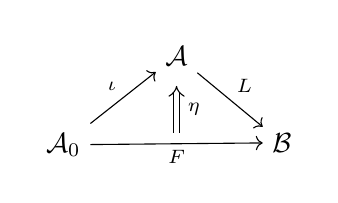
\begin{tikzpicture}[commutative diagrams/every diagram]
\matrix[matrix of math nodes, name=m]
{ & \mc A \\
\mc A_0 && \mc B \\
};
\path[commutative diagrams/.cd, every arrow, every label]
  (m-1-2) edge node {$L$} (m-2-3)
  (m-2-1) edge node {$\iota$} (m-1-2)
  (m-2-1) edge node[swap, name=D] {$F$} (m-2-3);
\draw[double,double equal sign distance,-implies,shorten >=4pt,shorten <=4pt] 
  (D) -- node[label={[label distance=-3pt]0:$\scriptstyle\eta$}] {} (m-1-2);
\end{tikzpicture}
\qquad\qquad
\begin{tikzcd}
& L\circ \iota \arrow[rd, dashed, "\sigma_\iota"] \\
F \arrow[ru, "\eta" ] \arrow[rr, "\alpha"'] && M\circ \iota
\end{tikzcd}
\]
Here $\sigma_F \colon L\iota \Rightarrow M\iota$ is the natural transformation with components $\sigma_\iota(a) = \sigma(\iota a) \colon L\iota(a) \to M\iota(a)$ for each $a\in \mc A_0$.   
Natural transformations were considered about, \eqref{eq:nat_trans}, and remember that they are (``vertically'') composed by composing their components, and so the condition becomes that for each $a\in\mc A_0$ we have $\alpha(a) = \sigma(\iota a) \circ \eta(a)$ or $\alpha_a = \sigma_{\iota a} \eta_a$ depending on notation.

(We note that the left diagram should be interpretted as a diagram in a 2-category: it says that $\eta$ is a natural transformation from $F$ to $L\iota$, and is \emph{not} meant to imply that the triangle commutes: if $L\iota=F$ then things are trivial.)

There is also the notion of a \emph{right Kan extension of $F$ along $\iota$}, written $R = \ran_\iota F$, which is a functor $R\colon \mc A \to \mc B$ and a natural transformation $\epsilon \colon R\iota \Rightarrow F$, universal in the sense that if $M\colon \mc A \to \mc B$ is any functor and $\mu \colon M\iota \Rightarrow F$ any natural transformation, there is a unique natural transformation $\delta \colon M \Rightarrow R$ with the right diagram commuting:
\[
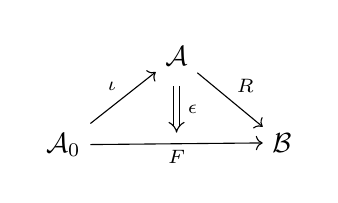
\begin{tikzpicture}[commutative diagrams/every diagram]
\matrix[matrix of math nodes, name=m]
{ & \mc A \\
\mc A_0 && \mc B \\
};
\path[commutative diagrams/.cd, every arrow, every label]
  (m-1-2) edge node {$R$} (m-2-3)
  (m-2-1) edge node {$\iota$} (m-1-2)
  (m-2-1) edge node[swap, name=D] {$F$} (m-2-3);
\draw[double,double equal sign distance,-implies,shorten >=4pt,shorten <=4pt] 
  (m-1-2) -- node[label={[label distance=-3pt]0:$\scriptstyle\epsilon$}] {} (D);
\end{tikzpicture}
\qquad\qquad
\begin{tikzcd}
& R\circ \iota \arrow[ld, "\epsilon"'] \\
F && M\circ \iota \arrow[ll, "\mu"] \arrow[dashed, lu, "\delta_\iota"']
\end{tikzcd}
\]
Again, here $\delta_\iota \colon M\iota \Rightarrow R\iota$ has components $\delta_\iota(a) = \delta(\iota a) \colon M\iota(a) \to R\iota(a)$ for each object $a\in\mc A_0$.

\begin{remark}
For our interests, our categories will be categories of Banach spaces or doolittle diagrams of Banach spaces.  So we are really working with ``enriched categories'' which for our purposes means that all functors and linear and contractive on morphism spaces, and the components of natural transformations are linear and contractive.
\end{remark}

We now give some examples, follow \cite[Section~II.VI.2]{KP_InterpolationFunctorsDuality}.

\subsection{Single doolittle diagram inclusion}

Let $\overline A \in \msf{BanDL}$ be a chosen doolittle diagram, and let $\mc A_0$ be the full subcategory of $\msf{BanDL}$ generated by this single object.  We consider a functor $F\colon \mc A_0 \to \mc B = \msf{Ban}$.  As explained in Section~\ref{sec:duality}, such a functor is equivalent to the data of a Banach space $A = F(\overline A)$ and a homomorphism $\mc B(\overline A) \to \mc B(A); \overline T \mapsto F(\overline T)$, that is, $A$ is a $\mc B(\overline A$)-module.

\subsubsection{Left Kan extension}

We show how to construct $\lan_\iota F = \lan_A$.
\[
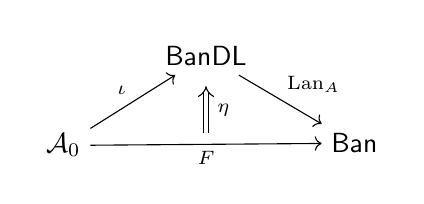
\begin{tikzpicture}[commutative diagrams/every diagram]
\matrix[matrix of math nodes, name=m]
{ & \msf{BanDL} \\
\mc A_0 && \msf{Ban} \\
};
\path[commutative diagrams/.cd, every arrow, every label]
  (m-1-2) edge node {$\lan_A$} (m-2-3)
  (m-2-1) edge node {$\iota$} (m-1-2)
  (m-2-1) edge node[swap, name=D] {$F$} (m-2-3);
\draw[double,double equal sign distance,-implies,shorten >=4pt,shorten <=4pt] 
  (D) -- node[label={[label distance=-3pt]0:$\scriptstyle\eta$}] {} (m-1-2);
\end{tikzpicture}
\qquad\qquad
\begin{tikzcd}
& L\circ \iota \arrow[rd, dashed, "\sigma_\iota"] \\
F \arrow[ru, "\eta" ] \arrow[rr, "\alpha"'] && M\circ \iota
\end{tikzcd}
\]
We claim that $\lan_A \overline X = \mc B(\overline A,\overline X) \proten_{\mc B(\overline A)} A$, the balanced tensor product.  Notice that $\mc B(\overline A,\overline X)$ is a right $\mc B(\overline A)$ module, with the action given by composition, and of course $A$ is a left module, so this makes sense.  The action of morphisms is given as follows.  For $\overline S \in\mc B(\overline X, \overline Y)$ we set $\lan_A \overline S \colon \mc B(\overline A,\overline X) \proten_{\mc B(\overline A)} A \to \mc B(\overline A,\overline Y) \proten_{\mc B(\overline A)} A$ to be $\overline R \otimes x \mapsto \overline S\overline R\otimes x$ on elementary tensors.  This is contractive for the projective tensor product, and the left composition by $\overline S$ commutes with the right module action, and so this maps drops to the balanced tensor product.

We now define $\eta \colon F \Rightarrow \lan_A \iota$.  As $\mc A_0$ has one object, we only need to consider the following situation:
\[ \begin{tikzcd}
\overline A \ar[d, "\overline T"] && F(\overline A)=A \ar[d, "F(\overline T)"] \ar[r, "\eta"] & \lan_A(\overline A) = \mc B(\overline A)\otimes_{\mc B(\overline A)} A = A 
\ar[d, "\lan_A(\overline T)"]
\\
\overline A && F(\overline A)=A \ar[r, "\eta"] & \lan_A(\overline A) = A
\end{tikzcd} \]
Here we confuse $\eta$ with the (single) component $\eta_{\overline A}$.  The isomorphism $\mc B(\overline A)\otimes_{\mc B(\overline A)} A = A$ is given by the module action, $\overline T \otimes x \mapsto \overline T\cdot x$, and hence $\lan_A(\overline T) = F(\overline T)$, namely the left module action.  Hence we can set $\eta=\id_A$.

Let us see that $\lan_A, \eta$ is universal.  Let $M\colon \msf{BanDL} \to \msf{Ban}$ be a functor and $\alpha \colon F \Rightarrow M\iota$ be a natural transformation.
That $\alpha$ is a natural transformation means that we have the commutative diagram
\begin{equation}\label{eq:alpha_nattrans}
\begin{tikzcd}
\overline A \ar[d, "\overline T"] && F(\overline A)=A \ar[d, "F(\overline T)"] \ar[r, "\alpha_{\overline A}"] & M(\overline A)
\ar[d, "M(\overline T)"]
\\
\overline A && F(\overline A)=A \ar[r, "\alpha_{\overline A}"] & M(\overline A)
\end{tikzcd} \end{equation}
We wish to define $\sigma \colon \lan_A \Rightarrow M$ to obtain $\alpha = \sigma_\iota \eta$.  Again, as $\mc A_0$ has a single object, we need only check that $\alpha_{\overline A} = \sigma_{\overline A} \circ \eta$, supressing the inclusion $\iota$ from our notation.  As $\eta = \eta_{\overline A}$ is the identity, we must have $\sigma_{\overline A} = \alpha_{\overline A}$.

For general $\overline X\in\msf{BanDL}$ we define the component
\[ \sigma_{\overline X} \colon \lan_A(\overline X) = \mc B(\overline A, \overline X) \otimes_{\mc B(\overline A)} A \to M(\overline X); \quad
\overline R \otimes x \mapsto M(\overline R) \alpha_{\overline A} (x). \]
This is well-defined, as $M(\overline R) \in \mc B(M(\overline A), M(\overline X))$, and for $\overline S\in\mc B(\overline A)$ we have that
\[ \overline R \overline S \otimes x - \overline R \otimes F(\overline S)x \mapsto M(\overline R) M(\overline S) \alpha_{\overline A}x - M(\overline R) \alpha_{\overline A} F(\overline S)x = 0, \]
as $\alpha$ is natural, \eqref{eq:alpha_nattrans}.  For $\overline T\in\mc B(\overline A)$, again by naturality, we have $\sigma_{\overline X}(\overline T\otimes x) \mapsto \alpha_{\overline A} F(\overline T)x$ and so $\sigma_{\overline A} = \alpha_{\overline A}$, as $\overline T\otimes x \cong F(\overline T)x$ under the isomorphism $\lan_A(\overline A) \cong A$.  We check that $\sigma$ is a natural transformation.  Consider the diagram
\[ \begin{tikzcd}
\overline X \ar[d, "\overline T"] && \lan_A(\overline X) \ar[r, "\sigma_{\overline X}"] \ar[d, "\lan_A(\overline T)"'] & M(\overline X) \ar[d, "M(\overline T)"]
\\
\overline Y && \lan_A(\overline X) \ar[r, "\sigma_{\overline Y}"'] & M(\overline Y)
\end{tikzcd} \]
For $\overline R\otimes x \in \lan_A(\overline X)$ we have that $M(\overline T) \sigma_{\overline X}(\overline R\otimes x) = M(\overline T) M(\overline R) \alpha_{\overline A}(x)$ while $\sigma_{\overline Y} \lan_A(\overline T)(\overline R\otimes x) = \sigma_{\overline Y}(\overline T\overline R\otimes x) = M(\overline T\overline R) \alpha_{\overline A}(x)$.  These agree, and so $\sigma$ is a natural transformation.

We show that $\sigma$ is unique.  For $\overline R\in\mc B(\overline A, \overline Y)$ and $x\in A$, for $F(\overline T)x \cong \overline T\otimes x \in \lan_A(\overline A)\cong A$ we have that $\lan_A(\overline R) F(\overline T)x = \overline R\overline T\otimes x = \overline R\otimes F(\overline T)x$ in the balanced tensor product.  That is, $\lan_A(\overline R) y = \overline R\otimes y$ for $y\in A$.  In the above diagram, take $\overline X = \overline A$, so that $M(\overline R)\alpha_{\overline A}y = M(\overline R)\sigma_{\overline A}y = \sigma_{\overline Y}\lan_A(\overline R)y = \sigma_{\overline Y}(\overline R\otimes y)$, and hence uniqueness of the definition of $\sigma$ follows.


\subsubsection{Right Kan extension}

We now consider $\ran_\iota F = \ran_A$.

\[
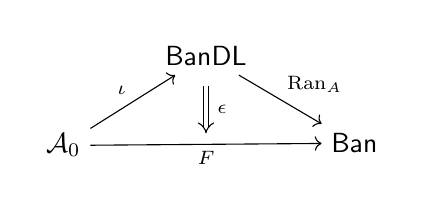
\begin{tikzpicture}[commutative diagrams/every diagram]
\matrix[matrix of math nodes, name=m]
{ & \msf{BanDL} \\
\mc A_0 && \msf{Ban} \\
};
\path[commutative diagrams/.cd, every arrow, every label]
  (m-1-2) edge node {$\ran_A$} (m-2-3)
  (m-2-1) edge node {$\iota$} (m-1-2)
  (m-2-1) edge node[swap, name=D] {$F$} (m-2-3);
\draw[double,double equal sign distance,-implies,shorten >=4pt,shorten <=4pt] 
  (m-1-2) -- node[label={[label distance=-3pt]0:$\scriptstyle\epsilon$}] {} (D);
\end{tikzpicture}
\qquad\qquad
\begin{tikzcd}
& \ran_A\iota \arrow[ld, "\epsilon"'] \\
F && M \iota \arrow[ll, "\mu"] \arrow[dashed, lu, "\delta_\iota"']
\end{tikzcd} \]

We claim that $\ran_A(\overline X) = {}_{\mc B(\overline A)}\mc B(\mc B(\overline X,\overline A), A)$ the space of left module maps; we have that $\mc B(\overline X,\overline A)$ is a $\mc B(\overline A)$-$\mc B(\overline X)$-bimodule by composition.  On morphisms, we have
\[ \ran_A(\overline T)(R) \colon \mc B(\overline Y,\overline A) \to A; \overline S \mapsto R(\overline S\circ\overline T)
\qquad (\overline T\in\mc B(\overline X, \overline Y), R\in{}_{\mc B(\overline A)}\mc B(\mc B(\overline X,\overline A), A)). \]
One checks that $\ran_A(\overline T)(R)$ is a module map.

As $\mc A_0$ has a single object, to define $\epsilon$ we need only specify $\epsilon_{\overline A} \colon \ran_A(\overline A) = {}_{\mc B(\overline A)}\mc B(\mc B(\overline A), A) \to A = F(\overline A)$.  Now, ${}_{\mc B(\overline A)}\mc B(\mc B(\overline A), A) \cong A$ as $R\in {}_{\mc B(\overline A)}\mc B(\mc B(\overline A), A)$ is determined by $R(\overline 1)$.  Again, we choose $\epsilon_{\overline A}$ to be the identity on $A$, once these identifications are made.

Consider now a functor $M \colon \msf{BanDL} \to \msf{Ban}$ along with a natural transformation $\mu \colon M\iota \Rightarrow F$.  So $\mu$ has a single component $\mu_{\overline A} \colon M(\overline A) \to A$ satisfying $F(\overline T) \mu_{\overline A} = \mu_{\overline A} M(\overline T)$ for each $\overline T \in \mc B(\overline A)$.  We seek to define $\delta \colon M \Rightarrow \ran_A$ with $\delta_{\overline A} = \epsilon_{\overline A} \delta_{\overline A} = \mu_{\overline A}$.

Let us proceed differently to the left case, and show why $\delta$ has to have a certain form.  For any $\overline X$ we need to have
\[ \begin{tikzcd}
\overline X \arrow[d, "\overline T"] && M(\overline X) \arrow[r, "\delta_{\overline X}"] \arrow[d, "M(\overline T)"'] & {}_{\mc B(\overline A)}\mc B(\mc B(\overline X,\overline A), A) \arrow[d, "\ran_A(\overline T)"]  \\
\overline A && M(\overline A) \arrow[r, "\delta_{\overline A}"] & \ran_A(\overline A) \cong A
\end{tikzcd} \]
Given the identifications we made above, $\ran_A(\overline T)$ is the map $R \mapsto R(\overline 1\circ \overline T) = R(\overline T)$.  Thus
\[ \delta_{\overline X}(\alpha)(\overline T) = \delta_{\overline A} M(\overline T)\alpha
= \mu_{\overline A} M(\overline T)\alpha
\qquad (\alpha\in M(\overline X), \overline T\in\mc B(\overline X,\overline A)). \]
Thus, if $\delta_{\overline X}$ exists, this uniquely defines it.  We have define $\delta_{\overline X}(\alpha) \in \mc B(\mc B(\overline X, \overline A), A)$; let us check that it is a module map.  For $\overline S\in\mc B(\overline A)$ we have that $\delta_{\overline X}(\alpha)(\overline S\overline T) = \mu_{\overline A} M(\overline S) M(\overline T) \alpha = F(\overline S) \mu_{\overline A} M(\overline T) \alpha = \overline S \cdot \delta_{\overline X}(\alpha)(\overline T)$, as required.

Given a general $\overline T \colon \overline X \to \overline Y$, for $\alpha\in M(\overline X)$ we have that
\begin{gather*}
\ran_A(\overline T) \delta_{\overline X}(\alpha) \colon \overline R \mapsto \delta_{\overline X}(\alpha)(\overline R\overline T) = \mu_{\overline A} M(\overline R) M(\overline T)(\alpha) \\
\delta_{\overline Y} M(\overline T)(\alpha) \colon \overline R \mapsto \mu_{\overline A} M(\overline R)\big( M(\overline T)\alpha \big),
\end{gather*}
which agree, showing that $\delta$ is natural.  Finally, for $\overline T\in\mc B(\overline A)$, we have $\delta_{\overline A}(\alpha)(\overline T) = \mu_{\overline A} M(\overline T)\alpha$ and so taking $\overline T=\overline 1$ gives $\delta_{\overline A}(\alpha) = \mu_{overline A} M(\overline 1)\alpha = \mu_{\overline A}\alpha$, whence $\delta_{\overline A} = \mu_{\overline A}$ as needed.

\subsubsection{Remarks}

There is some analogy with nuclear operators here.  Given $\overline T\otimes x \in \mc B(\overline A, \overline X) \proten_{\mc B(\overline A)} A \in \lan_A \overline X$ we can define
\[ R \colon \mc B(\overline X,\overline A) \to A; \quad \overline S \mapsto \overline S\circ\overline T \cdot x = F(\overline S)F(\overline T) x, \]
noticing that $\overline S\circ\overline T \in \mc B(\overline A)$.  Then $R$ is seen to be a module map, so $R\in\ran_A\overline X$.  Furthermore, the map $\overline T\otimes x \mapsto R$ is balanced, and so we obtain a contractive map $\lan_A \overline X \to \ran_A \overline X$.  For $\overline R\in\mc B(\overline X, \overline Y)$ we have $\lan_A \overline R \colon \overline T\otimes x \mapsto \overline R\overline T\otimes x$ which induces the map $R' \colon \overline S \mapsto F(\overline S\overline R\overline T)x = R(\overline S\overline R) = \ran_A\overline R (R)$.  So we have a natural transformation $\lan_A \Rightarrow \ran_A$.





\bibliographystyle{plain}
\bibliography{thebib.bib}

\end{document}
